\documentclass[fleqn,10pt]{wlscirep}\usepackage[]{graphicx}\usepackage[]{color}
%% maxwidth is the original width if it is less than linewidth
%% otherwise use linewidth (to make sure the graphics do not exceed the margin)
\makeatletter
\def\maxwidth{ %
  \ifdim\Gin@nat@width>\linewidth
    \linewidth
  \else
    \Gin@nat@width
  \fi
}
\makeatother

\definecolor{fgcolor}{rgb}{0.345, 0.345, 0.345}
\newcommand{\hlnum}[1]{\textcolor[rgb]{0.686,0.059,0.569}{#1}}%
\newcommand{\hlstr}[1]{\textcolor[rgb]{0.192,0.494,0.8}{#1}}%
\newcommand{\hlcom}[1]{\textcolor[rgb]{0.678,0.584,0.686}{\textit{#1}}}%
\newcommand{\hlopt}[1]{\textcolor[rgb]{0,0,0}{#1}}%
\newcommand{\hlstd}[1]{\textcolor[rgb]{0.345,0.345,0.345}{#1}}%
\newcommand{\hlkwa}[1]{\textcolor[rgb]{0.161,0.373,0.58}{\textbf{#1}}}%
\newcommand{\hlkwb}[1]{\textcolor[rgb]{0.69,0.353,0.396}{#1}}%
\newcommand{\hlkwc}[1]{\textcolor[rgb]{0.333,0.667,0.333}{#1}}%
\newcommand{\hlkwd}[1]{\textcolor[rgb]{0.737,0.353,0.396}{\textbf{#1}}}%
\let\hlipl\hlkwb

\usepackage{framed}
\makeatletter
\newenvironment{kframe}{%
 \def\at@end@of@kframe{}%
 \ifinner\ifhmode%
  \def\at@end@of@kframe{\end{minipage}}%
  \begin{minipage}{\columnwidth}%
 \fi\fi%
 \def\FrameCommand##1{\hskip\@totalleftmargin \hskip-\fboxsep
 \colorbox{shadecolor}{##1}\hskip-\fboxsep
     % There is no \\@totalrightmargin, so:
     \hskip-\linewidth \hskip-\@totalleftmargin \hskip\columnwidth}%
 \MakeFramed {\advance\hsize-\width
   \@totalleftmargin\z@ \linewidth\hsize
   \@setminipage}}%
 {\par\unskip\endMakeFramed%
 \at@end@of@kframe}
\makeatother

\definecolor{shadecolor}{rgb}{.97, .97, .97}
\definecolor{messagecolor}{rgb}{0, 0, 0}
\definecolor{warningcolor}{rgb}{1, 0, 1}
\definecolor{errorcolor}{rgb}{1, 0, 0}
\newenvironment{knitrout}{}{} % an empty environment to be redefined in TeX

\usepackage{alltt}

\usepackage{float}
\usepackage[english]{babel}

 
\setlength{\parindent}{0em} %  no indentation in paragraphs
\setlength{\parskip}{1em}


\title{Evaluating the Performance of Multiple Imputation by Chained Equations versus Complete Case Analysis through Simulations}

\author[1,*]{Faizan Khalid Mohsin}
\author[2]{Jasmine Ngyuen}
\author[2]{Hongyang Hu}
\author[2]{Nathan Taback}
\affil[1]{University of Toronto, Dalla Lana School of Public Health, Toronto, Canada}
\affil[2]{University of Toronto, Department of Statistical Sciences, Toronto, Canada}

\affil[*]{faizan.mohsin@mail.utoronto.ca}


%\keywords{Multiple Imputation by Chained Equations, Complete Case Analysis, Mixed-Effects Model}

\begin{abstract}

\textbf{Background:} The challenge of missing data is encountered by all disciplines of science. This is especially true when working with longitudinal data. One approach has been to use only those observations that have no missing data. This is called complete case analysis (CC). Another popular method is multiple imputation (MI) developed by Rubin. There are several implementations of multiple imputation and among them, multiple imputation by chained equations using predictive mean matching (MICE), has become popular. \textbf{Purpose:} We evaluate the performance of MICE and CC using simulated longitudinal data by methodologically introducing missing data. \textbf{Methodology:} Firstly, we simulate 100 data sets that are longitudinal in nature. We run mixed-effects model on the complete data sets and obtain the true estimate of the coefficients of the model. Now, in the simulated data we introduce three types of missingness: missing completely at random (MCAR), missing at random (MAR), and not missing at random (MNAR). We also methodologically introducing missingness at varying percentages. After this we use MICE and CC on the data sets and run a mixed-effects model to obtain estimates of the coefficients and also create 95\% confidence intervals. Finally, we compare these estimates to the true estimates of the modl. \textbf{Results:} We find that for both, MICE and CC, when missing data is at most 50\% and the missingness is either MCAR or MAR. Both missing data methods are very accurate. However, for MNAR, complete case analysis' confidence interval does capture the true estimate whereas MICE's does not. For over 50\% missing data, we did not even have enough complete cases to perform a complete case analysis. However, MICE did capture the true estimate even at 60\% missing data when the data was MCAR or MAR with the point estimates being very close to the true estimate. It did not, however, capture the true estimate in its confidence interval when the missing data was MNAR. \textbf{Conclusion:} Both methods perform equally well when missing data is less than 50\% with MICE being more precise (smaller CI and a smaller mse). However, when the missing data is MNAR, complete case analysis slightly outperforms MICE when missing data is less that 50\%, simply because it is much higher variance and thus bigger confidence intervals. Now, for over 50\% missing data there might not even be enough complete cases to perform a complete case analysis and so multiple imputation is very advantageous. Further, MICE performs very well even when missing data is over 50\% as long as the missingness is not MNAR. One possible reason CC and MI have similar performance for MAR is that the variables of our data sets were not correlated with one another, hence not allowing MICE to fully take advantage of this (which we know it can) and outperform CC which it theoretically should. 


\end{abstract}
\IfFileExists{upquote.sty}{\usepackage{upquote}}{}
\begin{document}

\flushbottom
\maketitle

\thispagestyle{empty}

\newpage

\section{Introduction}

These days, with more and more data, the problem of missing data is also increasing. Before the advent of computational power, and even today, for computational convenience, missing data is sometimes dealt with by simply keeping the observations with no missing data, that is, the complete cases and then analyzing this data set with only complete cases. This approach is called the complete case analysis. However, there have been made many advancements in the past several years and we will be discussing one of them known as multiple imputation (MI) by Rubin. Before we do so, we will describe the three different types of missing data. 

\subsection{Types of Missing Data}

Missing data is divided into three categories. The first is called missing completely at random (MCAR). As the name suggest, this type of missing data is missing completely at random \cite{allison2012handling}. There is no associative pattern between the missing data and the study or any aspect of the study. In such a case the missing data can simply be ignored. For example, if in a study where people's blood pressures are being measured and some people are unable to come due to a completely unrelated reason which has nothing to do with the person's blood pressure or anything else that we might be of interest in the study, such as relating to the person's age, gender, or ethnicity. A truly random reason such as being in an accident, or simply forgetting about it, would be considered missing completely at random.  

The second is called missing at random (MAR). This happens when the missing data depends on the other variables in the data set but not not the missing values \cite{allison2012handling}. For instance, if we are interested in people's blood pressure then if older people tend to have more missing values for their blood pressures then this could be a case where the missing data would be considered missing at random since the missingness depends on a person's age and not what their blood pressure is.  

The third is called not missing at random (NMAR or equivalently MNAR). This is when the missing data depends on the missing values themselves \cite{allison2012handling}. For example, in a study where people's blood pressure is being measured, the missing data will be considered not missing at random (NMAR) if the higher the person's blood pressure is, the higher the likelihood that he will not come in to have his blood pressure measured, hence causing the missingness of the blood pressure to depend on the blood pressure itself. If data is not missing at random, then it can have a significant impact on the study and can seriously bias the results. 

\subsection{Complete Case Analysis}

Complete case analysis is one of the methods to deal with missing data. Simply put, only those observations that have no missing data are retained in the data set. All others are deleted, hence it is called complete cases. This method is also sometimes known as listwise deletion. As the reader can surmise, in extreme cases when every observation has some missing data, all the data points would be deleted. Thus, it is typically recommended that variables with a lot of missing data be removed before hand. Further, ideally, the data sets should be large with little missing data so that the total percentage of observations deleted is low. Lastly, one possible issue of only keeping complete cases in the data set, is that it could introduce bias. For example, if the data is longitudinal, and there is missing data due to lack of follow-up for the last few time points because sicker people choose to discontinue (data being not missing at random). Deleting all such people and not using any of their data will introduce bias into the data set and any subsequent analysis. However, despite all of these issues, it is very attractive to use as it is very simple and easy to implement. Hence, one must be careful when using complete case analysis. 

\subsection{Multiple Imputation}

A more advanced method in which all the observations are kept is called multiple imputation. There are many multiple imputation methods, however all of them have three main steps \cite{dong2013principled}. The first step is to impute the missing values 'm' times creating 'm' complete data sets. Each data set is slightly different from the others, due to the randomness involved in the process, causing there to be variation between the competed data sets. The second step is to do the statistical analysis on each completed data set resulting into 'm' analyses. Hence, if we were estimating a parameter of a model, then we could have 'm' estimates, one from each data set. The third and last step is to combine all the 'm' analyses into the final result. Hence, for our 'm' estimates we could simply take their average \cite{yuan2010multiple, dong2013principled}. Figure \ref{fig:Faizan's_mi_fig} illustrates the multiple imputation method. 


\begin{figure}[H]
\centering
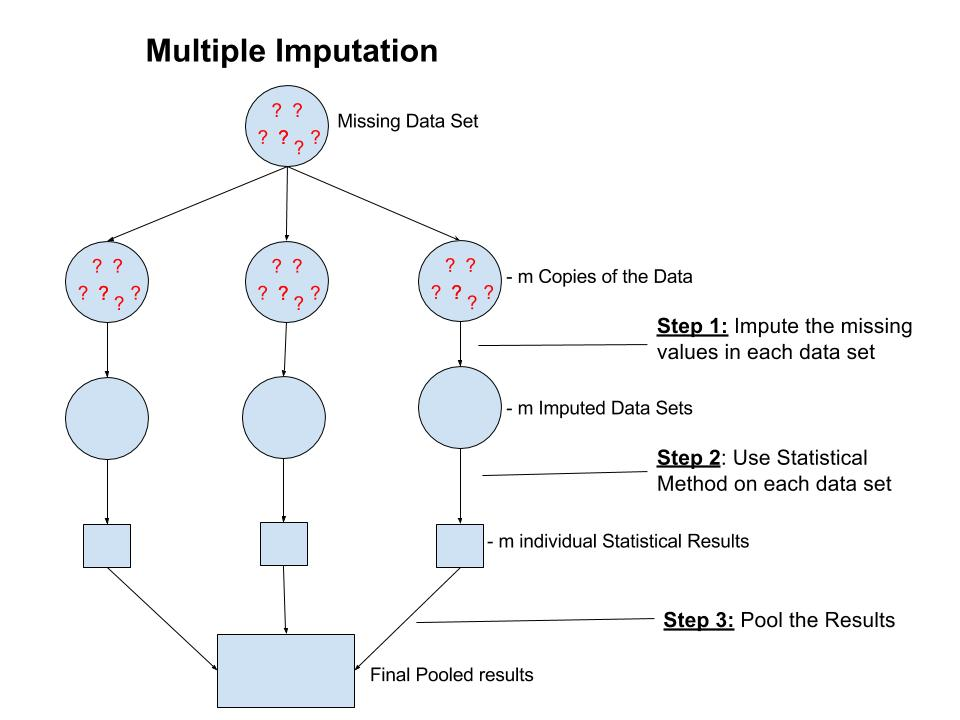
\includegraphics[width=\linewidth]{Faizan's_mi_fig}
\caption{Diagram illustrating the three main steps of the Multiple Imputation Method.}
\label{fig:Faizan's_mi_fig}
\end{figure}


An advantage of this method is that, to a degree, it accounts for the fact that the missing values are not known. I.e. it accounts for the fact that even though we may have an idea of the range of the possible values for the missing value, we are uncertain to what exact the value is. Hence, by creating 'm' different data sets we are introducing a new source of variation in our analysis which causes our estimate to have two sources that contribute towards it variance. Hence, two variance components. One is the usual variance of the data set, the other one is the new variance: the variance caused by the variation between data sets. The new variance component causes the estimate to have a higher variance. This accounts for the fact that we do not know what the missing value is. 

Further, if the assumption that the missing data is either MCAR or MAR and the three steps outlined above are done properly, then the estimates produced by the MI will have very desirable statistical properties. They will be consistent, almost asymptotically efficient and asymptotically normal \cite{allison2012handling}.


\subsection{Multiple Imputation by Chained Equations}

There are many methods as the reader can imagine how the missing values can be imputed in step one of the multiple imputation method. One popular semi-parametric method is called multiple imputation by chained equations\cite{Sterneb2393}. This is also the method we employed for doing multiple imputation. 

The simple idea behind multiple imputation by chained equations is performing a regression on the variable with missing values using the other variables as regressors and then using the predicted values plus a random error, from the regression of the missing value to be the new imputed value. And then some other variable with missing values is regressed on using all the other variables including the variable whose missing values were just imputed, and its missing values are imputed in the same fashion. This is done for all the variables with missing data and can be thought of as one cycle. This cycle is then repeated several times, typically ten or until convergence is reached for the missing values.\cite{Azur:2011, allison2012handling}

One clear advantage of this method is that if the variables in the data are correlated to one another then missing values in one variable could be fairly well estimated by the other variables through the successive regressions. However, on the flip side if the variables are not related to one another then performing regression would not substantially improve the estimates of the missing value. 

Further, we mentioned that we are using predictive mean matching for MICE. It is one of the options in the R "mice" package. We use this method because it is somewhat robust against the imputation model assumptions. For example the normality assumption, residuals being homoscedastic, and the associations being linear. Hence, predictive mean matching provides some robustness against the violation of these assumptions \cite{morris2014tuning}. 

We will investigate these advantages of multiple imputation by chained equations via evaluating its performance and will be comparing it to that of the complete case analysis. 


\section{Methods}

We will first give an overview of the entire process and then later go into depth for each step.  

\subsection{Overview of the Simulation and Analysis Process}

We simulate 100 data sets that are longitudinal in nature. We first introduce missing data that is missing completely at random (MCAR), then missing data that is missing at random (MAR) and finally, data that is not missing at random (MNAR). For each type of missing data, we introduce missingness at 20\%, 30\%, 40\% and 60\%. After this we use MICE and CC on the data sets to handle the missing data and then run a mixed-effects model to obtain 100 coefficient estimates for each (missing data) method. We take the average of these estimates to obtain the final coefficient estimates. We also create 95\% confidence intervals of these estimates. We then compare them to the true estimates that we obtain by running the mixed-effects model on the complete data sets (before introducing any missingness) obtaining 100 true coefficient estimates of which we again take the average and refer it to as the true coefficient estimates and create a 95\% confidence intervals for it as well. 

\begin{figure}[H]
\centering
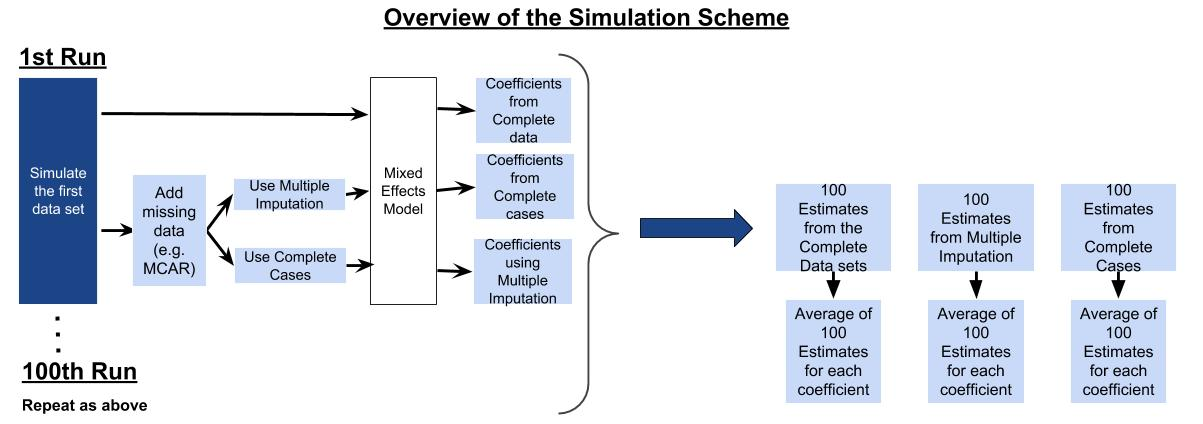
\includegraphics[width=\linewidth]{simulation_schema}
\caption{General overview of the simulation scheme.}
\label{fig:simulation_schema}
\end{figure}


\subsection{Simulating the Longitudinal data}

We create a longitudinal data set of 221 patients with a total of five time points (one baseline measurement and four follow-up measurements) with 1105 as the total number of data points. The variable of interest we will be using is FACIT-fatigue score (referred to simply as patient's fatigue score) which has the range 0-52 \cite{acaster2015qualitative}. We will also be simulating each person's age, gender, cancer stage and type of cancer. We did this so that the simulated data would resemble real world data sets. % The variables were inspired by a previous data set we had worked on. 

To simulate the longitudinal data we used the R software. 

\begin{itemize}

\item For the age variable we made it normally distributed with mean and standard deviation approximately 55 and 10 years, respectively. 
\item For the gender a binomial distribution was used with the probability of 80\% of being female and 20\% of being male. 
\item For cancer type, subjects can have one of five of the following cancers: "Breast", "Head and Neck", "Leukemia", "Prostate" or "Lung"  with females having the probability of 70\%, 10\%, 15\%, 0\%, and 5\% respectively for each of the cancers and males having the probability of 0\%, 10\%, 20\%, 60\% and 10\% respectively. As you can see females have zero probability of having prostate cancer and males have zero probability of having breast cancer. 
\item For the cancer stage, we made the higher cancer stages progressively more unlikely to occur. % the lower the probability of a person 
\item For the fatigue scores we made them normally distributed. To create the association between the patients' fatigue scores and the time points, we increased the mean fatigue score for each subsequent time point such that it would have a slope of 4. 

\end{itemize}

We illustrate the structure of the longitudinal data set below in Figure \ref{fig:sim_data_structure_scheme}. One can see that there are four levels to the data. 

\begin{figure}[H]
\centering
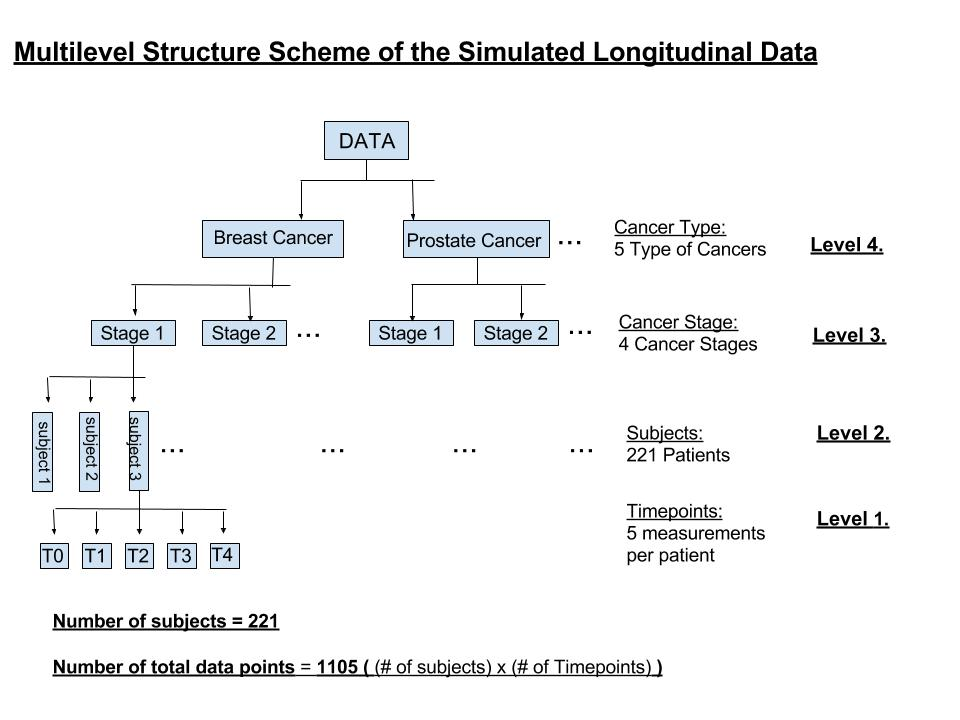
\includegraphics[width=\linewidth]{sim_data_structure_scheme}
\caption{Multilevel structure of the simulated data set.}
\label{fig:sim_data_structure_scheme}
\end{figure}

We also present in Figure \ref{fig:corr_sim_data} below the correlation structure of our simulated data between the different variables. As you can see that time point and the fatigue scores are relatively moderately correlated with a Pearson correlation coefficient of $r=0.58$. This is by design as you would recall that we set the fatigue scores to be normally distributed with increasing mean for each subsequent time point. Thus, fatigue scores and time points are correlated. You will also observe that the cancer type and the gender are also correlated with correlation coefficient of -0.71. This is also by design since only females can get breast cancer and only males can get prostrate cancer. For all the other variables they are uncorrelated to one another. 

\begin{figure}[H]
\centering
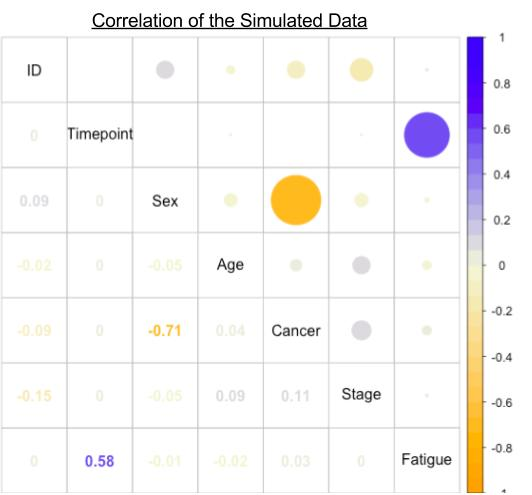
\includegraphics[width=\linewidth]{corr_sim_data}
\caption{Correlation structure of the simulated data set}
\label{fig:corr_sim_data}
\end{figure}


\subsection{Simulating the Missing Data}

After simulating the data we introduce three types of missingness. To simulate missing completely at random we simply randomly make the fatigue scores missing with all the fatigue scores having the same probability of being missing. To introduce missing at random we make the probability of a patient's fatigue score missing depend on the person's age. The higher the age, the greater the probability of having a missing value for the fatigue score. Lastly, for not missing at random we made the probability of having a missing value depend on the fatigues scores themselves with higher fatigue scores being more likely to be missing. We were also interested in testing how the two methods would perform if the MNAR was strong versus a weak relationship. For this, we simply linked more strongly higher probabilities of having missing fatigue scores to the higher fatigue scores. To introduce these three types of missing data we had three functions. By changing the probability of having missing values we could control what percentage of the data was missing. Hence, we were able to created data sets with 20\%, 30\%, 40\% and 60\% missing data for the variable of interest. For the reader's reference, sample code is provided in the appendix. 

\subsection{The Mixed Effect Model}

The mixed-effects model is used for modeling data with repeated measures. Hence, can be used to model repeated measures over time. The mixed effects model is:

$$\bold{y} = \bold{X \beta + Zu + \epsilon}$$


where:

\begin{itemize}
\item $\bold{y}$ is the vector of the variables of interest, with $E(\bold{y}) = \bold{X\beta}$;
\item $\beta$ is the vector of the coefficients of the fixed effects;
\item $u$ is the vector of random effects where $u \sim N(0, G)$;
\item $\epsilon$ is the vector of random errors with $\epsilon \sim N(0, R)$;
\item with $Cov(u,\epsilon) = 0$;
\item  $\bold{X}$ and $\bold{Z}$ are design matrices, where $\bold{X}$ is for the fixed effects and $\bold{Z}$ is for the random effects. 
\end{itemize}


To model the simulated longitudinal data using mixed-effects model we used the R package lme4. 


For our mixed-effect model, our response variable was the patient's fatigue score, which was treated as a continuous variable.The patients were treated as random effects over time. All the other covariates were treated as fixed effects: Cancer stage, cancer type, age, gender and the time points. The R code we used for our model was: 

$$lmer(FACTF\_Total \sim Timepoint + Age + Sex + CaDiagnosis\_Generalized + Stage\_Generalized + (Timepoint|ID))$$

Where FACTF\_Total is the fatigue score, CaDiagnosis\_Generalized is the type of cancer and Stage\_Generalized is the cancer stage. 

\subsection{Obtaining Estimates and Confidence Intervals from the 100 simulated data sets}

Once we simulated the 100 longitudinal data sets and then added missing data to them, we applied the complete case analysis and then multiple imputation by chained equations on the 100 data sets individually. Once the missing data was taken care of we applied the same mixed-effects model getting 100 estimates for each of the missing data methods. Then, to do the final step we took the average of the 100 estimates for the complete case analysis and we called this the final complete case point estimate. Similarly, we obtained the final MICE point estimate. Now, since we had the complete data sets we again fitted the mixed-effects model to the complete data sets obtaining 100 "true" estimates. Then again, simply took the average of the 100 "true" estimates to calculate the final "true" point estimate.  

To create the 95\% confidence interval of the MICE estimates of mixed-effects model we computed the 2.5\% and the 97.5\% quantiles of the 100 estimates we had obtained from the 100 simulations, with 2.5\% and 97.5\% quantiles being the lower and upper bounds of the confidence interval respectively. The 95\% confidence intervals of the complete case analysis estimates and the "true" estimates, were also constructed in the same manner. 

\section{Results}

\subsection{Comparing Multiple Imputation with Complete Case Analysis for different types, and over different percentages of missing data.}

We first present the results for 20\% and 30\% missing data with the missingness being missing completely at random, the most benign type. 

\begin{figure}[ht]
\centering
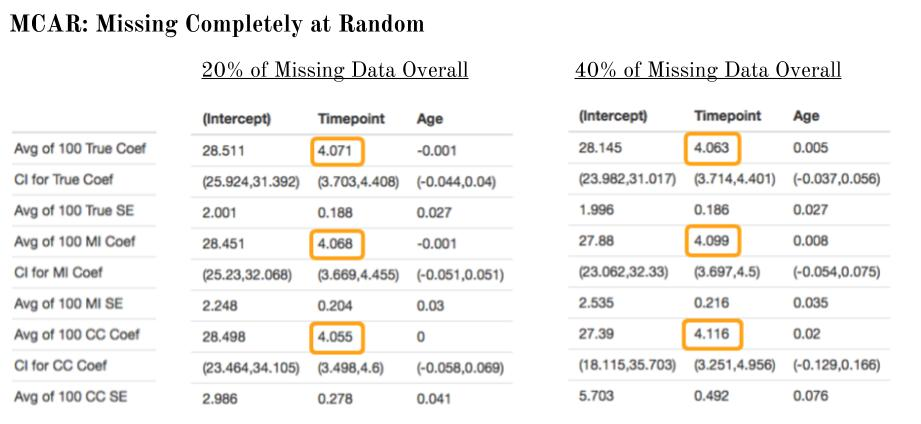
\includegraphics[width=\linewidth]{mcar_res_table}
\caption{Average of the 100 estimates of the coefficients obtained from the 100 simulated data for missing completely at random data. In this we are comparing the performance of complete case analysis and multiple imputation at the level of 20\% and 40\% missing data.}
\label{fig:mcar_res_table}
\end{figure}

From the above, one can see that for 20\% missing data the average of the 100 true coefficients (4.071), the average of the 100 MI coefficients (4.068), and the average of the 100 CC coefficients (4.055), are all very close (the estimates highlighted in orange). The same is true when the missing data is 40\%.

We shall now plot the results, drawing the 95\% confidence intervals as well and will also plot the results for 30\% missing data. 

\begin{figure}[H]
\centering
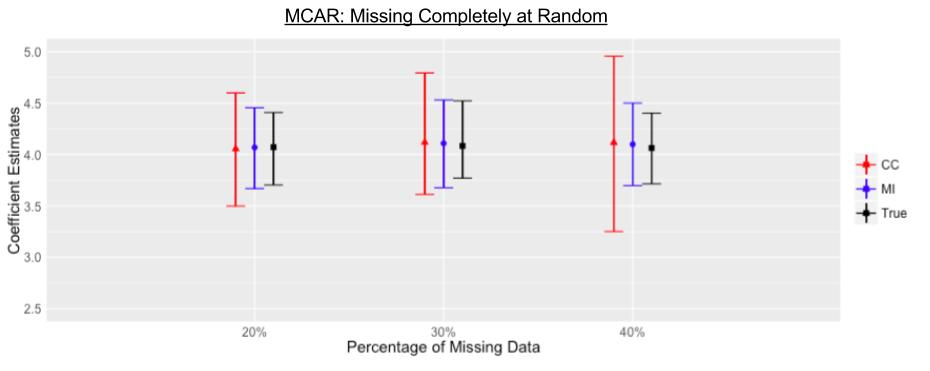
\includegraphics[width=\linewidth]{mcar_res_plot}
\caption{Performance of complete cases analysis and multiple imputation by chained equations for missing complete at random data.}
\label{fig:mcar_res_plot}
\end{figure}

One can see that the point estimates of MICE and CC are almost exactly the same as the true coefficient estimate. Further, their confidence intervals overlap, with complete case analysis having larger confidence intervals than multiple imputation, especially when 40\% of the data is missing. Hence, one clear advantage of multiple imputation over CC is that it is more accurate, especialy when missing data is high. 

We repeated the above but with the missing data now being missing at random (MAR), where the missingness of the fatigue scores depend on the age of the person. 


\begin{figure}[H]
\centering
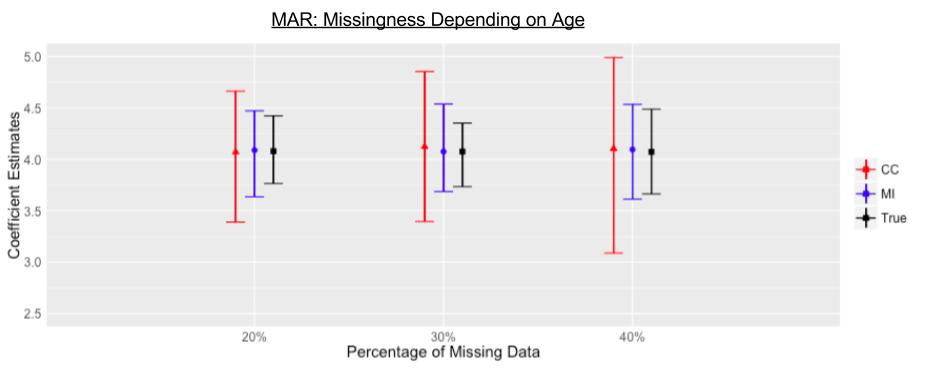
\includegraphics[width=\linewidth]{mar_res_plot}
\caption{Performance of complete case analysis and multiple imputation with missing at random data.}
\label{fig:mar_res_plot}
\end{figure}

Here, we see, perhaps a bit surprisingly, that even though the data is missing at random, complete case analysis performs as well as multiple imputation. Theoretocally, complete case analysis should be worse off than multiple imputation, as it should only be able to handle data that is missing completely at random. 

Now, we introduce missing data that is not missing at random (NMAR), with the probability of the fatigue score missing depending on the fatigue score itself. We designed this so that higher fatigue scores were more likely to be missing. After running the simulation 100 times we plot the results below. 

\begin{figure}[H]
\centering
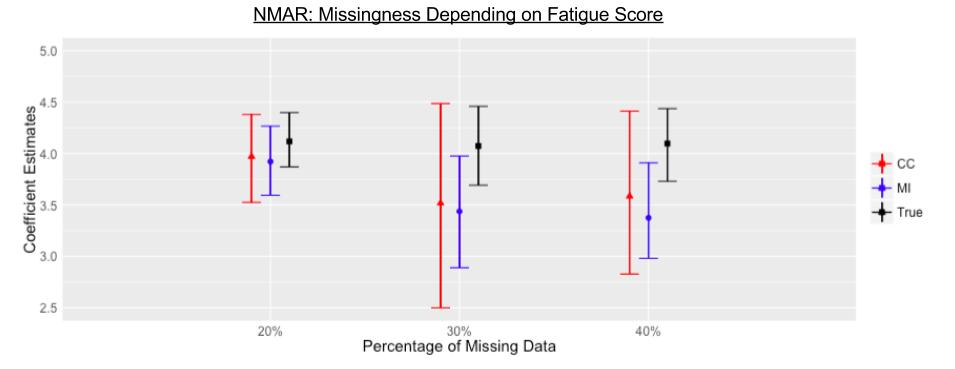
\includegraphics[width=\linewidth]{nmar_res_plot}
\caption{Performance of complete case analysis and multiple imputation for not missing at random data at different percentages of missing data.}
\label{fig:nmar_res_plot}
\end{figure}

We see that even for 20\% missing data, the point estimates of the two missing data methods are not as accurate as before. Then, when the missingness increases to 30\% and 40\% the point estimates are way off and multiple imputation's confidence intervals do not even contain the true point estimates of the coefficient. 


\subsection{Comparing the performance of Complete Cases and Multiple Imputation for weak vs. strong Not Missing at Random data and evaluating the performance of MI for 60\% of missing data.}

We will now see how complete case analysis and multiple imputation perform when there is a strong MNAR pattern for the missing data and when there is a weak one. Both weak and strong MNAR are for 40\% missing data. We have plotted the results below in Figure \ref{fig:nmar_weak_vs_strong}.   

\begin{figure}[H]
\centering
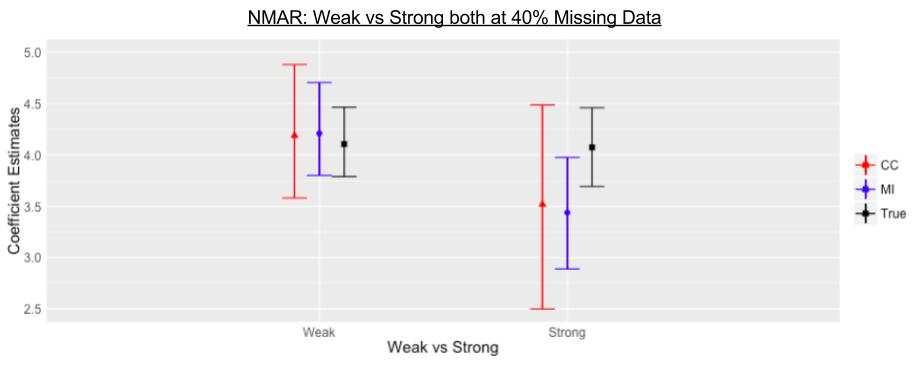
\includegraphics[width=\linewidth]{nmar_weak_vs_strong}
\caption{Performance of complete case analysis and multiple imputation for weak and strong NMAR with 40\% missing data.}
\label{fig:nmar_weak_vs_strong}
\end{figure}

We see that when the MNAR is weak, the performance of complete case analysis and multiple imputation are both very accurate even with 40\% missing data. However, both perform poorly when there is a strong MNAR missing data pattern, with complete case analysis doing slightly better that multiple imputation as its confidence interval captures the true coefficients point estimate and its point estimate is slightly closer to the true estimate than that of the multiple imputation. 

We tried to compare the performance of multiple imputation and complete case analysis for 60\% missing data. However, there were not enough complete cases to perform a complete case analysis. Thus, we only looked at how well multiple imputation performs for the different types of missing data, when 60\% of the data is missing.     

\begin{figure}[H]
\centering
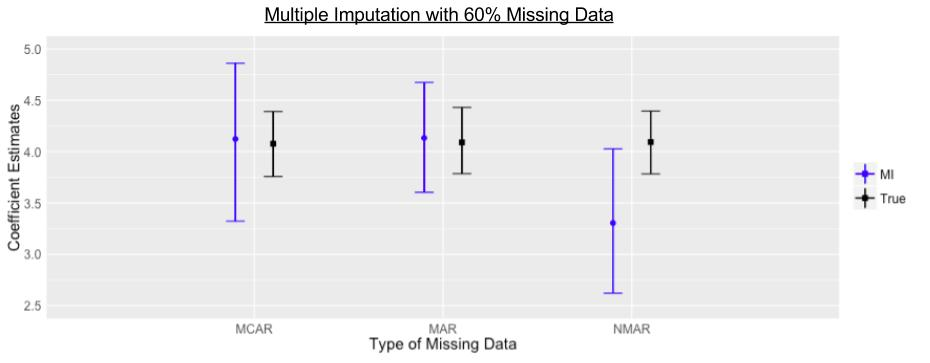
\includegraphics[width=\linewidth]{mi_60per_missing_plot}
\caption{Performance of multiple imputation for MCAR, MAR and NMAR missing data at 60\% missingness.}
\label{fig:mi_60per_missing_plot}
\end{figure}

From Figure \ref{fig:mi_60per_missing_plot} we see that even when the missing data is very high, 60\% as long as the missing data is missing completely at random or missing at random then multiple imputation performs very well. However, when the missing data is not missing at random then, multiple imputation does not perform very well. 


\section{Discussion}

Firstly, one of the most interesting finding we found was that for MAR, in terms of point estimate of the coefficients, complete case analysis and multiple imputation performed equally well (see Figure \ref{fig:mar_res_plot}). This is surprising, since theoretically, multiple imputation is able to handle MAR but complete case analysis is not. However, when we simulated the data we made all the variables uncorrelated, except time point and fatigue scores, and gender and cancer type. Hence, as the algorithm of MICE uses to its advantage the correlation between variables, and there was no such relationship for MICE to exploit, both methods yielded similar results for MAR data. This result does make sense and we found one other paper by Mukaka et. al 2016 where researchers using real world data, found CC and MI to perform equally well \cite{mukaka2016using}. 

Further, for missing data under 50\% and with the MCAR and MAR conditions, we found that both MICE and CC confidence intervals capture the true estimate with MICE's point estimate being very slightly closer to the true estimate compared to CC (see Figure \ref{fig:mcar_res_plot} and Figure \ref{fig:mar_res_plot}, respectively). Also, the CC coefficient estimates have much larger variance compared to MICE and hence much larger confidence intervals. And from our simulation study we can see that for MCAR and MAR, both MICE and CC give unbiased estimates. Therefore, MICE would has smaller mse compared to CC making MICE the better method inspite of the point estimates of the two methods having similarly good performance. 

Now for NMAR, both MICE and CC estimates are biased and the bias becomes progressively worse as the percentage of missing data increases (see Figure \ref{fig:nmar_res_plot}). However, when the missing data is 20\% both MICE and CC perform reasonably well as they are able to capture the true estimate in their confidence intervals. Now when the missing data percentage increases, the CC estimate's confidence interval, which is much larger compared to MICE's, is able to capture the true estimate of the coefficient, whereas MICE's does not (although, MICE's confidence interval does overlap with that of the true estimate's confidence interval). Also, the point estimate for the complete cases was slightly closer to the true estimate than that of MICE. Therefore, both methods do not perform very well when the data is NMAR. Though, NMAR has less of an impact when there is little missing data. 

Further, we also wanted to see how MICE and CC would perform when the NMAR was weak. By NMAR being weak, we mean that the probability for the Y value to be missing is weakly related to the value of Y (the varaible of interst, fatigue score in our case). For this we kept the missing data at 40\%. From Figure \ref{fig:nmar_weak_vs_strong} we see that MICE actually performs very reasonably when NMAR is weak and performs very badly when it is strong. In fact CC also happens to perform reasonably well. So even if the missing data is NMAR, but there is a weak relationship between the value of the variable of interest and its probability of missing, MICE and CC perform quite well. 

Now, when missing data is over 50\%, we did not even have enough complete cases to perform a complete case analysis. Where we can see a clear advantage for MICE. Further, MICE was even able to capture the true estimate even at 60\% missing data when the data was MCAR or MAR with the point estimates being very close to the true estimate, as seen in Figure \ref{fig:mi_60per_missing_plot}. It did not however, capture the true estimate in its confidence interval when the missing data was MNAR. This said, it is actually not advised to perform imputation when missing data is over 50\%. However, as can be seen, if the missing data is MCAR or MAR and there can not be made any improvement on the missingness of the data set, then for practical reasons, one could use MICE. These results are indeed very intersting. Especially, the fact that MICE predicts the true point estimate accurately with little to no bias for MCAR and MAR. Also, our results show that MICE is not able to handle NMAR data with 60\% data, as one would expect.


\textbf{Final Conclusion:} Both methods perform equally well when missing data is less than 50\% with MICE being more precise (smaller CI). However, when the missing data is MNAR, complete case analysis somewhat technically outperforms MICE due to its larger confidence interval. For over 50\% missing data, there might not be enough complete cases to perform a complete case analysis. MICE, in our particular case, performs very well even when missing data is over 50\% as long as the missing data is not MNAR. 


\bibliography{sample}

% \noindent LaTeX formats citations and references automatically using the bibliography records in your .bib file, which you can edit via the project menu. Use the cite command for an inline citation, e.g.  \cite{Figueredo:2009dg}.

% \section*{Acknowledgements (not compulsory)}

% Acknowledgements should be brief, and should not include thanks to anonymous referees and editors, or effusive comments. Grant or contribution numbers may be acknowledged.

\section*{Author contributions statement}

F.K.M. conceived the research question, methodology and experiments. F.K.M., J.N. and H.H. conducted the experiments and the analysis. The final results and analysis were reviewed by all the authors F.K.M., J.N., H.H. and N.T.. F.K.M. wrote and reviewed the manuscript. 

\section*{Additional information}

\textbf{Competing financial interests} 

The authors declare no competing interests.

% Figures and tables can be referenced in LaTeX using the ref command, e.g. Figure \ref{fig:stream} and Table \ref{tab:example}.

\textbf{Source Code}

To obtain the complete source code for this study, please contact the authors directly. 

\section*{Appendix}

\textbf{Sample Code}

First we will provide sample code of the script and then code for the helper functions.

\begin{knitrout}
\definecolor{shadecolor}{rgb}{0.969, 0.969, 0.969}\color{fgcolor}\begin{kframe}
\begin{alltt}
\hlcom{###################### Script Code #####################################}

\hlcom{#### First simulate the data }
\hlstd{sim1} \hlkwb{=} \hlkwd{sim_data}\hlstd{(dataset,} \hlkwc{p_female}\hlstd{=}\hlnum{.8}\hlstd{,} \hlkwc{p0}\hlstd{=p0,} \hlkwc{p1}\hlstd{=p1,} \hlkwc{p2}\hlstd{=p2,} \hlkwc{p3}\hlstd{=p3,} \hlkwc{p4}\hlstd{=p4)}
\hlcom{# Look at the correlations among the variables of the correlated data}
\hlstd{MM} \hlkwb{<-} \hlkwd{cor}\hlstd{(sim1,} \hlkwc{use} \hlstd{=} \hlstr{"pairwise.complete.obs"}\hlstd{)}
\hlkwd{corrplot}\hlstd{(MM,} \hlkwc{method}\hlstd{=}\hlstr{"circle"}\hlstd{)}
\hlkwd{corrplot.mixed}\hlstd{(MM)}

\hlcom{# MCAR 20% overall missing data}
\hlstd{p_absent} \hlkwb{=} \hlkwd{c}\hlstd{(}\hlnum{.4}\hlstd{,} \hlnum{.05}\hlstd{,} \hlnum{.05}\hlstd{)}
\hlstd{p_missing} \hlkwb{=} \hlkwd{c}\hlstd{(}\hlnum{.2}\hlstd{,} \hlnum{.2}\hlstd{,} \hlnum{.2}\hlstd{,} \hlnum{.1}\hlstd{)}
\hlcom{# Simulate missing data according to the different p's for MCAR}
\hlstd{sim1_data} \hlkwb{=} \hlkwd{mcar_final}\hlstd{(sim1, p_absent,} \hlkwc{p} \hlstd{= p_missing)}
\hlcom{# Find total Missing % and Missing % at Each Timepoint for MCAR}
\hlkwd{perc_miss_vec}\hlstd{(sim1_data)}
\hlkwd{perc_miss}\hlstd{(sim1_data)}
\hlcom{# See how the results are affected for the MCAR }
\hlstd{Test_MCAR_20per} \hlkwb{=} \hlkwd{simulation_mcar}\hlstd{(dataset,} \hlkwc{n.sim} \hlstd{= n_sim,} \hlkwc{m} \hlstd{=} \hlnum{5}\hlstd{,} \hlkwc{p_absent} \hlstd{= p_absent,}
                                  \hlkwc{p} \hlstd{= p_missing,} \hlkwc{p_female}\hlstd{=}\hlnum{.8}\hlstd{,} \hlkwc{p0}\hlstd{=p0,} \hlkwc{p1}\hlstd{=p1,} \hlkwc{p2}\hlstd{=p2,}
                                  \hlkwc{p3}\hlstd{=p3,} \hlkwc{p4}\hlstd{=p4)}
\hlstd{Test_MCAR_20}


\hlcom{# MAR 30% overall missing data}
\hlstd{p_absent} \hlkwb{=} \hlkwd{c}\hlstd{(}\hlnum{.2}\hlstd{,} \hlnum{.1}\hlstd{,} \hlnum{.05}\hlstd{)}
\hlstd{p_missing} \hlkwb{=} \hlkwd{c}\hlstd{(}\hlnum{.1}\hlstd{,} \hlnum{.1}\hlstd{,} \hlnum{.1}\hlstd{,} \hlnum{.4}\hlstd{)}
\hlcom{# Simulate missing data according to the p's for MAR}
\hlstd{sim1_data} \hlkwb{=} \hlkwd{mar_final}\hlstd{(sim1,} \hlkwc{p_absent} \hlstd{= p_absent, p_missing, pattern_age)}
\hlcom{# Find total Missing % and Missing % at Each Timepoint for MAR}
\hlstd{perc_miss_vec_results} \hlkwb{=} \hlkwd{perc_miss_vec}\hlstd{(sim1_data); perc_miss_vec_results}
\hlkwd{perc_miss}\hlstd{(sim1_data)}
\hlcom{# See how the results are affected for the MAR }
\hlstd{Test_MAR_30perc} \hlkwb{=} \hlkwd{simulation_mar}\hlstd{(dataset,} \hlkwc{n.sim} \hlstd{= n_sim,} \hlkwc{m} \hlstd{=} \hlnum{5}\hlstd{,} \hlkwc{p_absent} \hlstd{= p_absent,}
                                 \hlkwc{p_missing} \hlstd{= p_missing,} \hlkwc{pattern} \hlstd{= pattern_age,}
                                 \hlkwc{p_female}\hlstd{=}\hlnum{.8}\hlstd{,} \hlkwc{p0}\hlstd{=p0,} \hlkwc{p1}\hlstd{=p1,} \hlkwc{p2}\hlstd{=p2,} \hlkwc{p3}\hlstd{=p3,} \hlkwc{p4}\hlstd{=p4)}
\hlstd{Test_MAR_30perc}


\hlcom{# Strong NMAR 20% overall Missing data}
\hlstd{p_absent} \hlkwb{=}  \hlkwd{c}\hlstd{(}\hlnum{.3}\hlstd{,} \hlnum{.05}\hlstd{,} \hlnum{.05}\hlstd{)}
\hlstd{p_missing} \hlkwb{=} \hlkwd{c}\hlstd{(}\hlnum{.001}\hlstd{,} \hlnum{.001}\hlstd{,} \hlnum{.05}\hlstd{,} \hlnum{.3}\hlstd{)}
\hlcom{# Simulate missing data according to the p's for NMAR}
\hlstd{sim1_data} \hlkwb{=} \hlkwd{nmar_final}\hlstd{(sim1, p_absent, p_missing, pattern)}
\hlcom{# Find total Missing % and Missing % at Each Timepoint for MAR}
\hlkwd{perc_miss}\hlstd{(sim1_data)}
\hlkwd{perc_miss_vec}\hlstd{(sim1_data)}
\hlcom{# See how the results are affected for the MAR }
\hlstd{Test_strong_NMAR_20per} \hlkwb{=} \hlkwd{simulation_nmar}\hlstd{(dataset,} \hlkwc{n.sim} \hlstd{= n_sim,} \hlkwc{m} \hlstd{=} \hlnum{5}\hlstd{,} \hlkwc{p_absent}\hlstd{=p_absent,}
                                         \hlstd{p_missing,} \hlkwc{pattern} \hlstd{= pattern,} \hlkwc{p_female}\hlstd{=}\hlnum{.8}\hlstd{,} \hlkwc{p0}\hlstd{=p0,}
                                         \hlkwc{p1}\hlstd{=p1,} \hlkwc{p2}\hlstd{=p2,} \hlkwc{p3}\hlstd{=p3,} \hlkwc{p4}\hlstd{=p4)}
\hlstd{Test_NMAR_20per}


\hlcom{# Weak NMAR 30% overall Missing data}
\hlstd{p_absent} \hlkwb{=}  \hlkwd{c}\hlstd{(}\hlnum{.3}\hlstd{,} \hlnum{.1}\hlstd{,} \hlnum{.1}\hlstd{)}
\hlstd{p_missing} \hlkwb{=} \hlkwd{c}\hlstd{(}\hlnum{.2}\hlstd{,} \hlnum{.25}\hlstd{,} \hlnum{.3}\hlstd{,} \hlnum{.4}\hlstd{)}
\hlcom{# Simulate missing data according to the p's for NMAR}
\hlstd{sim1_data} \hlkwb{=} \hlkwd{nmar_final}\hlstd{(sim1, p_absent, p_missing, pattern)}
\hlcom{# Find total Missing % and Missing % at Each Timepoint for MAR}
\hlkwd{perc_miss}\hlstd{(sim1_data)}
\hlkwd{perc_miss_vec}\hlstd{(sim1_data)}
\hlcom{# See how the results are affected for the MAR }
\hlstd{Test_weak_NMAR_30per} \hlkwb{=} \hlkwd{simulation_nmar}\hlstd{(dataset,} \hlkwc{n.sim} \hlstd{= n_sim,} \hlkwc{m} \hlstd{=} \hlnum{5}\hlstd{,} \hlkwc{p_absent} \hlstd{= p_absent,}
                                       \hlstd{p_missing,} \hlkwc{pattern} \hlstd{= pattern,} \hlkwc{p_female}\hlstd{=}\hlnum{.8}\hlstd{,} \hlkwc{p0}\hlstd{=p0,}
                                       \hlkwc{p1}\hlstd{=p1,} \hlkwc{p2}\hlstd{=p2,} \hlkwc{p3}\hlstd{=p3,} \hlkwc{p4}\hlstd{=p4)}
\hlstd{Test_NMAR_30per}


\hlcom{###################### Helper Functions #####################################}

\hlcom{######################## Simulating the data #################################}

\hlcom{######}
\hlcom{###### Function that simulates the data}
\hlcom{######}

\hlstd{sim_data} \hlkwb{=} \hlkwa{function}\hlstd{(}\hlkwc{data}\hlstd{,} \hlkwc{p_female}\hlstd{=}\hlnum{.8}\hlstd{,} \hlkwc{p0}\hlstd{=}\hlkwd{rep}\hlstd{(}\hlnum{1}\hlstd{,}\hlnum{52}\hlstd{),} \hlkwc{p1}\hlstd{=}\hlkwd{rep}\hlstd{(}\hlnum{1}\hlstd{,}\hlnum{52}\hlstd{),}
                    \hlkwc{p2}\hlstd{=}\hlkwd{rep}\hlstd{(}\hlnum{1}\hlstd{,}\hlnum{52}\hlstd{),} \hlkwc{p3}\hlstd{=}\hlkwd{rep}\hlstd{(}\hlnum{1}\hlstd{,}\hlnum{52}\hlstd{),} \hlkwc{p4}\hlstd{=}\hlkwd{rep}\hlstd{(}\hlnum{1}\hlstd{,}\hlnum{52}\hlstd{))\{}

  \hlstd{f_vec} \hlkwb{=} \hlnum{0}\hlopt{:}\hlnum{52}

  \hlcom{# female is 1 and male is 0 }
  \hlcom{# breast = 1, Head and neck = 2, Leukemia = 3, Prostrate = 4, Lung = 5 }
  \hlcom{#cancer = c("Breast", "Head and Neck", "Leukemia", "Prostate", "Lung")}

  \hlstd{cancer} \hlkwb{=} \hlkwd{c}\hlstd{(}\hlnum{1}\hlstd{,} \hlnum{2}\hlstd{,} \hlnum{3}\hlstd{,} \hlnum{4}\hlstd{,} \hlnum{5}\hlstd{)}

  \hlstd{j} \hlkwb{=} \hlnum{1}
  \hlkwa{while} \hlstd{(j} \hlopt{<} \hlkwd{nrow}\hlstd{(data) )\{}

    \hlstd{a1} \hlkwb{=} \hlkwd{sample}\hlstd{(}\hlkwd{c}\hlstd{(}\hlnum{1}\hlstd{,}\hlnum{0}\hlstd{),} \hlkwc{size} \hlstd{=} \hlnum{1}\hlstd{,} \hlkwc{prob} \hlstd{=} \hlkwd{c}\hlstd{(p_female,} \hlnum{1}\hlopt{-}\hlstd{p_female))}
    \hlstd{a2} \hlkwb{=} \hlkwd{round}\hlstd{(}\hlkwd{rnorm}\hlstd{(}\hlkwc{n} \hlstd{=} \hlnum{1}\hlstd{,} \hlkwc{mean} \hlstd{=} \hlnum{54.93}\hlstd{,} \hlkwc{sd} \hlstd{=} \hlnum{9.829}\hlstd{))}
    \hlstd{a3} \hlkwb{=} \hlkwa{if} \hlstd{(a1} \hlopt{==} \hlnum{1}\hlstd{)} \hlkwd{sample}\hlstd{(cancer,} \hlkwc{size} \hlstd{=} \hlnum{1}\hlstd{,} \hlkwc{prob} \hlstd{=} \hlkwd{c}\hlstd{(}\hlnum{0.7}\hlstd{,} \hlnum{.10}\hlstd{,} \hlnum{.15}\hlstd{,} \hlnum{0}\hlstd{,} \hlnum{.05}\hlstd{) )}
          \hlkwa{else}  \hlkwd{sample}\hlstd{(cancer,} \hlkwc{size} \hlstd{=} \hlnum{1}\hlstd{,} \hlkwc{prob} \hlstd{=} \hlkwd{c}\hlstd{(}\hlnum{0}\hlstd{,} \hlnum{.10}\hlstd{,} \hlnum{.20}\hlstd{,} \hlnum{.60}\hlstd{,} \hlnum{.10}\hlstd{) )}
    \hlstd{a4} \hlkwb{=} \hlkwd{sample}\hlstd{(}\hlnum{1}\hlopt{:}\hlnum{4}\hlstd{,} \hlkwc{size} \hlstd{=} \hlnum{1}\hlstd{,} \hlkwc{prob} \hlstd{=} \hlkwd{c}\hlstd{(}\hlnum{43}\hlstd{,} \hlnum{49}\hlstd{,} \hlnum{59}\hlstd{,} \hlnum{19}\hlstd{) )}

    \hlstd{a} \hlkwb{=} \hlkwd{c}\hlstd{(a1, a2, a3, a4)}

    \hlstd{data[j,} \hlkwd{c}\hlstd{(}\hlnum{3}\hlstd{,} \hlnum{4}\hlstd{,} \hlnum{5}\hlstd{,} \hlnum{6}\hlstd{)]} \hlkwb{=} \hlstd{a}
    \hlstd{data[j}\hlopt{+}\hlnum{1}\hlstd{,} \hlkwd{c}\hlstd{(}\hlnum{3}\hlstd{,} \hlnum{4}\hlstd{,} \hlnum{5}\hlstd{,} \hlnum{6}\hlstd{)]} \hlkwb{=} \hlstd{a}
    \hlstd{data[j}\hlopt{+}\hlnum{2}\hlstd{,} \hlkwd{c}\hlstd{(}\hlnum{3}\hlstd{,} \hlnum{4}\hlstd{,} \hlnum{5}\hlstd{,} \hlnum{6}\hlstd{)]} \hlkwb{=} \hlstd{a}
    \hlstd{data[j}\hlopt{+}\hlnum{3}\hlstd{,} \hlkwd{c}\hlstd{(}\hlnum{3}\hlstd{,} \hlnum{4}\hlstd{,} \hlnum{5}\hlstd{,} \hlnum{6}\hlstd{)]} \hlkwb{=} \hlstd{a}
    \hlstd{data[j}\hlopt{+}\hlnum{4}\hlstd{,} \hlkwd{c}\hlstd{(}\hlnum{3}\hlstd{,} \hlnum{4}\hlstd{,} \hlnum{5}\hlstd{,} \hlnum{6}\hlstd{)]} \hlkwb{=} \hlstd{a}

    \hlstd{data[j,} \hlkwd{ncol}\hlstd{(data)]} \hlkwb{=} \hlkwd{sample}\hlstd{(f_vec,} \hlkwc{size} \hlstd{=} \hlnum{1}\hlstd{,} \hlkwc{prob} \hlstd{= p0)}
    \hlstd{data[j}\hlopt{+}\hlnum{1}\hlstd{,} \hlkwd{ncol}\hlstd{(data)]} \hlkwb{=} \hlkwd{sample}\hlstd{(f_vec,} \hlkwc{size} \hlstd{=} \hlnum{1}\hlstd{,} \hlkwc{prob} \hlstd{= p1)}
    \hlstd{data[j}\hlopt{+}\hlnum{2}\hlstd{,} \hlkwd{ncol}\hlstd{(data)]} \hlkwb{=} \hlkwd{sample}\hlstd{(f_vec,} \hlkwc{size} \hlstd{=} \hlnum{1}\hlstd{,} \hlkwc{prob} \hlstd{= p2)}
    \hlstd{data[j}\hlopt{+}\hlnum{3}\hlstd{,} \hlkwd{ncol}\hlstd{(data)]} \hlkwb{=} \hlkwd{sample}\hlstd{(f_vec,} \hlkwc{size} \hlstd{=} \hlnum{1}\hlstd{,} \hlkwc{prob} \hlstd{= p3)}
    \hlstd{data[j}\hlopt{+}\hlnum{4}\hlstd{,} \hlkwd{ncol}\hlstd{(data)]} \hlkwb{=} \hlkwd{sample}\hlstd{(f_vec,} \hlkwc{size} \hlstd{=} \hlnum{1}\hlstd{,} \hlkwc{prob} \hlstd{= p4)}

    \hlstd{j} \hlkwb{=} \hlstd{j} \hlopt{+} \hlnum{5}

  \hlstd{\}}

  \hlstd{data}
\hlstd{\}}

\hlcom{# # Test}
\hlcom{# f_vec = 0:52}
\hlcom{# p0 = dnorm(f_vec, mean = 27, sd = 10)}
\hlcom{# p1 = dnorm(f_vec, mean = 35, sd = 9)}
\hlcom{# p2 = dnorm(f_vec, mean = 42, sd = 10)}
\hlcom{# p3 = dnorm(f_vec, mean = 45, sd = 10)}
\hlcom{# p4 = dnorm(f_vec, mean = 47, sd = 10)}
\hlcom{# sim1 = sim_data(data = simdata, p_female = .83, p0=p0, p1=p1, p2=p2, p3=p3, p4=p4)}


\hlcom{###################### Introducing missingness to data. #######################}


\hlcom{######}
\hlcom{###### Function that creates MCAR data at the rate of p_i% at each Timepoint i.}
\hlcom{######}

\hlstd{mcar_final} \hlkwb{=} \hlkwa{function}\hlstd{(}\hlkwc{data}\hlstd{,} \hlkwc{p_absent}\hlstd{,} \hlkwc{p}\hlstd{,} \hlkwc{seed}\hlstd{)\{}

  \hlstd{n} \hlkwb{=} \hlkwd{nrow}\hlstd{(data)}

  \hlkwa{for} \hlstd{(i} \hlkwa{in} \hlnum{1}\hlopt{:}\hlstd{n)\{}

    \hlstd{f_score} \hlkwb{=} \hlstd{data[i,}\hlkwd{ncol}\hlstd{(data)]}
    \hlstd{p1} \hlkwb{=} \hlnum{0}
    \hlstd{p2} \hlkwb{=} \hlnum{0}
    \hlstd{p3} \hlkwb{=} \hlnum{0}


    \hlkwa{if} \hlstd{(data[i, ]}\hlopt{$}\hlstd{Timepoint} \hlopt{==} \hlnum{1}\hlstd{)\{}
      \hlstd{data[i,}\hlkwd{ncol}\hlstd{(data)]}\hlkwb{=}\hlkwd{sample}\hlstd{(}\hlkwd{c}\hlstd{(}\hlnum{NA}\hlstd{, f_score),} \hlkwc{size} \hlstd{=} \hlnum{1}\hlstd{,} \hlkwc{prob} \hlstd{=} \hlkwd{c}\hlstd{(p[}\hlnum{1}\hlstd{],} \hlnum{1}\hlopt{-}\hlstd{p[}\hlnum{1}\hlstd{]))}
    \hlstd{\}}

    \hlkwa{if} \hlstd{(data[i, ]}\hlopt{$}\hlstd{Timepoint} \hlopt{==} \hlnum{2}\hlstd{)\{}

      \hlkwa{if}\hlstd{(}\hlkwd{is.na}\hlstd{(data}\hlopt{$}\hlstd{FACTF_Total[i}\hlopt{-}\hlnum{1}\hlstd{]))\{}
        \hlstd{p1} \hlkwb{=} \hlstd{p_absent[}\hlnum{1}\hlstd{]}
      \hlstd{\}}

      \hlstd{data[i,}\hlkwd{ncol}\hlstd{(data)]}\hlkwb{=}\hlkwd{sample}\hlstd{(}\hlkwd{c}\hlstd{(}\hlnum{NA}\hlstd{, f_score),} \hlkwc{size} \hlstd{=} \hlnum{1}\hlstd{,} \hlkwc{prob} \hlstd{=} \hlkwd{c}\hlstd{(p[}\hlnum{2}\hlstd{]} \hlopt{+} \hlstd{p1 ,} \hlnum{1} \hlopt{-} \hlstd{(p1}\hlopt{+}\hlstd{p[}\hlnum{2}\hlstd{]) ))}
    \hlstd{\}}

    \hlkwa{if} \hlstd{(data[i, ]}\hlopt{$}\hlstd{Timepoint} \hlopt{==} \hlnum{3}\hlstd{)\{}

      \hlkwa{if}\hlstd{(}\hlkwd{is.na}\hlstd{(data}\hlopt{$}\hlstd{FACTF_Total[i}\hlopt{-}\hlnum{1}\hlstd{]))\{}
        \hlstd{p1} \hlkwb{=} \hlstd{p_absent[}\hlnum{1}\hlstd{]}
      \hlstd{\}}

      \hlkwa{if}\hlstd{(}\hlkwd{is.na}\hlstd{(data}\hlopt{$}\hlstd{FACTF_Total[i}\hlopt{-}\hlnum{2}\hlstd{]))\{}
        \hlstd{p2} \hlkwb{=} \hlstd{p_absent[}\hlnum{2}\hlstd{]}
      \hlstd{\}}
      \hlstd{pp} \hlkwb{=} \hlstd{p1} \hlopt{+} \hlstd{p2}

      \hlstd{data[i,}\hlkwd{ncol}\hlstd{(data)]}\hlkwb{=}\hlkwd{sample}\hlstd{(}\hlkwd{c}\hlstd{(}\hlnum{NA}\hlstd{, f_score),} \hlkwc{size} \hlstd{=}  \hlnum{1}\hlstd{,} \hlkwc{prob} \hlstd{=} \hlkwd{c}\hlstd{(pp}\hlopt{+}\hlstd{p[}\hlnum{3}\hlstd{],} \hlnum{1}\hlopt{-}\hlstd{(pp}\hlopt{+}\hlstd{p[}\hlnum{3}\hlstd{])))}
    \hlstd{\}}

    \hlkwa{if} \hlstd{(data[i, ]}\hlopt{$}\hlstd{Timepoint} \hlopt{==} \hlnum{4}\hlstd{)\{}


      \hlkwa{if}\hlstd{(}\hlkwd{is.na}\hlstd{(data}\hlopt{$}\hlstd{FACTF_Total[i}\hlopt{-}\hlnum{1}\hlstd{]))\{}
        \hlstd{p1} \hlkwb{=} \hlstd{p_absent[}\hlnum{1}\hlstd{]}
      \hlstd{\}}

      \hlkwa{if}\hlstd{(}\hlkwd{is.na}\hlstd{(data}\hlopt{$}\hlstd{FACTF_Total[i}\hlopt{-}\hlnum{2}\hlstd{]))\{}
        \hlstd{p2} \hlkwb{=} \hlstd{p_absent[}\hlnum{2}\hlstd{]}
      \hlstd{\}}

      \hlkwa{if}\hlstd{(}\hlkwd{is.na}\hlstd{(data}\hlopt{$}\hlstd{FACTF_Total[i}\hlopt{-}\hlnum{3}\hlstd{]))\{}
        \hlstd{p3} \hlkwb{=} \hlstd{p_absent[}\hlnum{3}\hlstd{]}
      \hlstd{\}}

      \hlstd{pp} \hlkwb{=} \hlstd{p1} \hlopt{+} \hlstd{p2} \hlopt{+} \hlstd{p3}


      \hlstd{data[i,}\hlkwd{ncol}\hlstd{(data)]}\hlkwb{=}\hlkwd{sample}\hlstd{(}\hlkwd{c}\hlstd{(}\hlnum{NA}\hlstd{, f_score),} \hlkwc{size} \hlstd{=} \hlnum{1}\hlstd{,} \hlkwc{prob} \hlstd{=} \hlkwd{c}\hlstd{(pp}\hlopt{+}\hlstd{p[}\hlnum{4}\hlstd{],} \hlnum{1}\hlopt{-}\hlstd{(pp}\hlopt{+}\hlstd{p[}\hlnum{4}\hlstd{])))}
    \hlstd{\}}

  \hlstd{\}}
  \hlstd{data}
\hlstd{\}}

\hlcom{# Test}
\hlcom{# vecdata = mcar_final(data = sim2, p_absent = c(.1, .1, .1), p = c(.4, .4, .4, .4) )}
\hlcom{# perc_miss_vec(vecdata)}
\hlcom{# perc_miss(vecdata)}



\hlcom{######}
\hlcom{###### Final Function that creates MAR data at the rate of p%}
\hlcom{######}

\hlcom{# Creating Missing at Random Condition. Assumption: the missingness is associated with Age}
\hlstd{mar_final}\hlkwb{<-}\hlkwa{function}\hlstd{(}\hlkwc{df}\hlstd{,} \hlkwc{p_absent}\hlstd{,} \hlkwc{p_missing}\hlstd{,} \hlkwc{pattern}\hlstd{)\{}
  \hlkwa{for}\hlstd{(i} \hlkwa{in} \hlnum{1}\hlopt{:}\hlkwd{nrow}\hlstd{(df))\{}

    \hlkwa{if}\hlstd{(df}\hlopt{$}\hlstd{Timepoint[i]} \hlopt{!=} \hlnum{0}\hlstd{) \{}

      \hlstd{pp} \hlkwb{=} \hlnum{0}
      \hlstd{p1} \hlkwb{=} \hlnum{0}
      \hlstd{p2} \hlkwb{=} \hlnum{0}
      \hlstd{p3} \hlkwb{=} \hlnum{0}

      \hlkwa{if} \hlstd{(data[i, ]}\hlopt{$}\hlstd{Timepoint} \hlopt{==} \hlnum{2}\hlstd{)\{}

        \hlkwa{if}\hlstd{(}\hlkwd{is.na}\hlstd{(data}\hlopt{$}\hlstd{FACTF_Total[i}\hlopt{-}\hlnum{1}\hlstd{]))\{}
          \hlstd{pp} \hlkwb{=} \hlstd{p_absent[}\hlnum{1}\hlstd{]}
        \hlstd{\}}
      \hlstd{\}}

      \hlkwa{if} \hlstd{(data[i, ]}\hlopt{$}\hlstd{Timepoint} \hlopt{==} \hlnum{3}\hlstd{)\{}

        \hlkwa{if}\hlstd{(}\hlkwd{is.na}\hlstd{(data}\hlopt{$}\hlstd{FACTF_Total[i}\hlopt{-}\hlnum{1}\hlstd{]))\{}
          \hlstd{p1} \hlkwb{=} \hlstd{p_absent[}\hlnum{1}\hlstd{]}
        \hlstd{\}}

        \hlkwa{if}\hlstd{(}\hlkwd{is.na}\hlstd{(data}\hlopt{$}\hlstd{FACTF_Total[i}\hlopt{-}\hlnum{2}\hlstd{]))\{}
          \hlstd{p2} \hlkwb{=} \hlstd{p_absent[}\hlnum{2}\hlstd{]}
        \hlstd{\}}
        \hlstd{pp} \hlkwb{=} \hlstd{p1} \hlopt{+} \hlstd{p2}
      \hlstd{\}}

      \hlkwa{if} \hlstd{(data[i, ]}\hlopt{$}\hlstd{Timepoint} \hlopt{==} \hlnum{4}\hlstd{)\{}

        \hlkwa{if}\hlstd{(}\hlkwd{is.na}\hlstd{(data}\hlopt{$}\hlstd{FACTF_Total[i}\hlopt{-}\hlnum{1}\hlstd{]))\{}
          \hlstd{p1} \hlkwb{=} \hlstd{p_absent[}\hlnum{1}\hlstd{]}
        \hlstd{\}}

        \hlkwa{if}\hlstd{(}\hlkwd{is.na}\hlstd{(data}\hlopt{$}\hlstd{FACTF_Total[i}\hlopt{-}\hlnum{2}\hlstd{]))\{}
          \hlstd{p2} \hlkwb{=} \hlstd{p_absent[}\hlnum{2}\hlstd{]}
        \hlstd{\}}

        \hlkwa{if}\hlstd{(}\hlkwd{is.na}\hlstd{(data}\hlopt{$}\hlstd{FACTF_Total[i}\hlopt{-}\hlnum{3}\hlstd{]))\{}
          \hlstd{p3} \hlkwb{=} \hlstd{p_absent[}\hlnum{3}\hlstd{]}
        \hlstd{\}}

        \hlstd{pp} \hlkwb{=} \hlstd{p1} \hlopt{+} \hlstd{p2} \hlopt{+} \hlstd{p3}
      \hlstd{\}}

      \hlkwa{if}\hlstd{(pattern[}\hlnum{1}\hlstd{,}\hlnum{1}\hlstd{]}\hlopt{<=}\hlstd{df}\hlopt{$}\hlstd{Age[i]} \hlopt{&&} \hlstd{df}\hlopt{$}\hlstd{Age[i]}\hlopt{<=}\hlstd{pattern[}\hlnum{1}\hlstd{,}\hlnum{2}\hlstd{])\{}
        \hlcom{# Removing the data for for certain chances if the 0<= fatigue score <=12 }
        \hlstd{df}\hlopt{$}\hlstd{FACTF_Total[i]}\hlkwb{<-}\hlkwd{sample}\hlstd{(}\hlkwd{c}\hlstd{(}\hlnum{NA}\hlstd{, df}\hlopt{$}\hlstd{FACTF_Total[i]),} \hlkwc{size} \hlstd{=} \hlnum{1}\hlstd{,}
                                  \hlkwc{prob} \hlstd{=} \hlkwd{c}\hlstd{(p_missing[}\hlnum{1}\hlstd{]} \hlopt{+} \hlstd{pp ,} \hlnum{1}\hlopt{-}\hlstd{(pp} \hlopt{+} \hlstd{p_missing[}\hlnum{1}\hlstd{])))}
        \hlkwa{next}
      \hlstd{\}}
      \hlkwa{if}\hlstd{(pattern[}\hlnum{2}\hlstd{,}\hlnum{1}\hlstd{]}\hlopt{<=}\hlstd{df}\hlopt{$}\hlstd{Age[i]} \hlopt{&&} \hlstd{df}\hlopt{$}\hlstd{Age[i]}\hlopt{<=}\hlstd{pattern[}\hlnum{2}\hlstd{,}\hlnum{2}\hlstd{])\{}
        \hlcom{# Removing the data for for certain chances if the 13<= fatigue score <=25 }
        \hlstd{df}\hlopt{$}\hlstd{FACTF_Total[i]}\hlkwb{<-}\hlkwd{sample}\hlstd{(}\hlkwd{c}\hlstd{(}\hlnum{NA}\hlstd{, df}\hlopt{$}\hlstd{FACTF_Total[i]),} \hlkwc{size} \hlstd{=} \hlnum{1}\hlstd{,}
                                  \hlkwc{prob} \hlstd{=} \hlkwd{c}\hlstd{(p_missing[}\hlnum{2}\hlstd{]} \hlopt{+} \hlstd{pp,} \hlnum{1} \hlopt{-}\hlstd{(pp} \hlopt{+} \hlstd{p_missing[}\hlnum{2}\hlstd{])))}
        \hlkwa{next}
      \hlstd{\}}
      \hlkwa{if}\hlstd{(pattern[}\hlnum{3}\hlstd{,}\hlnum{1}\hlstd{]}\hlopt{<=}\hlstd{df}\hlopt{$}\hlstd{Age[i]} \hlopt{&&} \hlstd{df}\hlopt{$}\hlstd{Age[i]}\hlopt{<=}\hlstd{pattern[}\hlnum{3}\hlstd{,}\hlnum{2}\hlstd{])\{}
        \hlcom{# Removing the data for for certain chances if the 26<= fatigue score <=38 }
        \hlstd{df}\hlopt{$}\hlstd{FACTF_Total[i]}\hlkwb{<-}\hlkwd{sample}\hlstd{(}\hlkwd{c}\hlstd{(}\hlnum{NA}\hlstd{, df}\hlopt{$}\hlstd{FACTF_Total[i]),} \hlkwc{size} \hlstd{=} \hlnum{1}\hlstd{,}
                                  \hlkwc{prob} \hlstd{=} \hlkwd{c}\hlstd{(p_missing[}\hlnum{3}\hlstd{]} \hlopt{+} \hlstd{pp ,} \hlnum{1}\hlopt{-}\hlstd{(pp} \hlopt{+} \hlstd{p_missing[}\hlnum{3}\hlstd{])))}
        \hlkwa{next}
      \hlstd{\}}
      \hlkwa{if}\hlstd{(pattern[}\hlnum{4}\hlstd{,}\hlnum{1}\hlstd{]}\hlopt{<=}\hlstd{df}\hlopt{$}\hlstd{Age[i]} \hlopt{&&} \hlstd{df}\hlopt{$}\hlstd{Age[i]}\hlopt{<=}\hlstd{pattern[}\hlnum{4}\hlstd{,}\hlnum{2}\hlstd{])\{}
        \hlcom{# Removing the data for for certain chances if the 39<= fatigue score <=52 }
        \hlstd{df}\hlopt{$}\hlstd{FACTF_Total[i]}\hlkwb{<-}\hlkwd{sample}\hlstd{(}\hlkwd{c}\hlstd{(}\hlnum{NA}\hlstd{, df}\hlopt{$}\hlstd{FACTF_Total[i]),} \hlkwc{size} \hlstd{=} \hlnum{1}\hlstd{,}
                                  \hlkwc{prob} \hlstd{=} \hlkwd{c}\hlstd{(p_missing[}\hlnum{4}\hlstd{]} \hlopt{+} \hlstd{pp ,} \hlnum{1}\hlopt{-}\hlstd{(pp} \hlopt{+} \hlstd{p_missing[}\hlnum{4}\hlstd{])))}
      \hlstd{\}}

    \hlstd{\}}

  \hlstd{\}}
  \hlstd{df}
\hlstd{\}}

\hlcom{## Test}
\hlcom{# mar_data1 = mar_final(sim2)}
\hlcom{# perc_miss_vec(mar_data1)}
\hlcom{# perc_miss(mar_data1)}


\hlcom{######}
\hlcom{###### Function that creates Not Missing at Random data.}
\hlcom{######}

\hlcom{# Creating Not Missing at Random Condition. }
\hlcom{# Assumption: the missingness is associated with Total Fatigue Score}
\hlstd{nmar_final} \hlkwb{=} \hlkwa{function}\hlstd{(}\hlkwc{data}\hlstd{,} \hlkwc{p_absent}\hlstd{,} \hlkwc{p_missing}\hlstd{,}  \hlkwc{pattern}\hlstd{)\{}


  \hlstd{n} \hlkwb{=} \hlkwd{nrow}\hlstd{(data)}

  \hlkwa{for} \hlstd{(i} \hlkwa{in} \hlnum{1}\hlopt{:}\hlstd{n)\{}

    \hlstd{p1} \hlkwb{=} \hlnum{0}
    \hlstd{p2} \hlkwb{=} \hlnum{0}
    \hlstd{p3} \hlkwb{=} \hlnum{0}
    \hlstd{pp} \hlkwb{=} \hlnum{0}

    \hlkwa{if} \hlstd{(data[i, ]}\hlopt{$}\hlstd{Timepoint} \hlopt{==} \hlnum{2}\hlstd{)\{}

      \hlkwa{if}\hlstd{(}\hlkwd{is.na}\hlstd{(data}\hlopt{$}\hlstd{FACTF_Total[i}\hlopt{-}\hlnum{1}\hlstd{]))\{}
        \hlstd{p1} \hlkwb{=} \hlstd{p_absent[}\hlnum{1}\hlstd{]}
      \hlstd{\}}

      \hlstd{pp} \hlkwb{=} \hlstd{p1}

    \hlstd{\}}

    \hlkwa{if} \hlstd{(data[i, ]}\hlopt{$}\hlstd{Timepoint} \hlopt{==} \hlnum{3}\hlstd{)\{}

      \hlkwa{if}\hlstd{(}\hlkwd{is.na}\hlstd{(data}\hlopt{$}\hlstd{FACTF_Total[i}\hlopt{-}\hlnum{1}\hlstd{]))\{}
        \hlstd{p1} \hlkwb{=} \hlstd{p_absent[}\hlnum{1}\hlstd{]}
      \hlstd{\}}

      \hlkwa{if}\hlstd{(}\hlkwd{is.na}\hlstd{(data}\hlopt{$}\hlstd{FACTF_Total[i}\hlopt{-}\hlnum{2}\hlstd{]))\{}
        \hlstd{p2} \hlkwb{=} \hlstd{p_absent[}\hlnum{2}\hlstd{]}
      \hlstd{\}}

      \hlstd{pp} \hlkwb{=} \hlstd{p1} \hlopt{+} \hlstd{p2}



    \hlstd{\}}

    \hlkwa{if} \hlstd{(data[i, ]}\hlopt{$}\hlstd{Timepoint} \hlopt{==} \hlnum{4}\hlstd{)\{}


      \hlkwa{if}\hlstd{(}\hlkwd{is.na}\hlstd{(data}\hlopt{$}\hlstd{FACTF_Total[i}\hlopt{-}\hlnum{1}\hlstd{]))\{}
        \hlstd{p1} \hlkwb{=} \hlstd{p_absent[}\hlnum{1}\hlstd{]}
      \hlstd{\}}

      \hlkwa{if}\hlstd{(}\hlkwd{is.na}\hlstd{(data}\hlopt{$}\hlstd{FACTF_Total[i}\hlopt{-}\hlnum{2}\hlstd{]))\{}
        \hlstd{p2} \hlkwb{=} \hlstd{p_absent[}\hlnum{2}\hlstd{]}
      \hlstd{\}}

      \hlkwa{if}\hlstd{(}\hlkwd{is.na}\hlstd{(data}\hlopt{$}\hlstd{FACTF_Total[i}\hlopt{-}\hlnum{3}\hlstd{]))\{}
        \hlstd{p3} \hlkwb{=} \hlstd{p_absent[}\hlnum{3}\hlstd{]}
      \hlstd{\}}

      \hlstd{pp} \hlkwb{=} \hlstd{p1} \hlopt{+} \hlstd{p2} \hlopt{+} \hlstd{p3}

    \hlstd{\}}

    \hlkwa{if}\hlstd{(data}\hlopt{$}\hlstd{Timepoint[i]} \hlopt{!=} \hlnum{0}\hlstd{)\{}

      \hlkwa{if}\hlstd{(pattern[}\hlnum{1}\hlstd{,}\hlnum{1}\hlstd{]}\hlopt{<=}\hlstd{data}\hlopt{$}\hlstd{FACTF_Total[i]} \hlopt{&&} \hlstd{data}\hlopt{$}\hlstd{FACTF_Total[i]}\hlopt{<=}\hlstd{pattern[}\hlnum{1}\hlstd{,}\hlnum{2}\hlstd{])\{}
        \hlcom{# Removing the data for for certain chances if the 0<= fatigue score <=12 }
        \hlstd{data}\hlopt{$}\hlstd{FACTF_Total[i]}\hlkwb{<-}\hlkwd{sample}\hlstd{(}\hlkwd{c}\hlstd{(data}\hlopt{$}\hlstd{FACTF_Total[i],}\hlnum{NA}\hlstd{),} \hlkwc{size} \hlstd{=} \hlnum{1}\hlstd{,}
                                    \hlkwc{prob} \hlstd{=} \hlkwd{c}\hlstd{(}\hlnum{1}\hlopt{-}\hlstd{(pp}\hlopt{+} \hlstd{p_missing[}\hlnum{1}\hlstd{]), pp} \hlopt{+} \hlstd{p_missing[}\hlnum{1}\hlstd{]))}
        \hlkwa{next}
      \hlstd{\}}
      \hlkwa{if}\hlstd{(pattern[}\hlnum{2}\hlstd{,}\hlnum{1}\hlstd{]}\hlopt{<=}\hlstd{data}\hlopt{$}\hlstd{FACTF_Total[i]} \hlopt{&&} \hlstd{data}\hlopt{$}\hlstd{FACTF_Total[i]}\hlopt{<=}\hlstd{pattern[}\hlnum{2}\hlstd{,}\hlnum{2}\hlstd{])\{}
        \hlcom{# Removing the data for for certain chances if the 13<= fatigue score <=25 }
        \hlstd{data}\hlopt{$}\hlstd{FACTF_Total[i]}\hlkwb{<-}\hlkwd{sample}\hlstd{(}\hlkwd{c}\hlstd{(data}\hlopt{$}\hlstd{FACTF_Total[i],}\hlnum{NA}\hlstd{),} \hlkwc{size} \hlstd{=} \hlnum{1}\hlstd{,}
                                    \hlkwc{prob} \hlstd{=} \hlkwd{c}\hlstd{(}\hlnum{1}\hlopt{-}\hlstd{( pp} \hlopt{+} \hlstd{p_missing[}\hlnum{2}\hlstd{]), pp} \hlopt{+} \hlstd{p_missing[}\hlnum{2}\hlstd{]))}
        \hlkwa{next}
      \hlstd{\}}
      \hlkwa{if}\hlstd{(pattern[}\hlnum{3}\hlstd{,}\hlnum{1}\hlstd{]}\hlopt{<=}\hlstd{data}\hlopt{$}\hlstd{FACTF_Total[i]} \hlopt{&&} \hlstd{data}\hlopt{$}\hlstd{FACTF_Total[i]}\hlopt{<=}\hlstd{pattern[}\hlnum{3}\hlstd{,}\hlnum{2}\hlstd{])\{}
        \hlcom{# Removing the data for for certain chances if the 26<= fatigue score <=38 }
        \hlstd{data}\hlopt{$}\hlstd{FACTF_Total[i]}\hlkwb{<-}\hlkwd{sample}\hlstd{(}\hlkwd{c}\hlstd{(data}\hlopt{$}\hlstd{FACTF_Total[i],}\hlnum{NA}\hlstd{),} \hlkwc{size} \hlstd{=} \hlnum{1}\hlstd{,}
                                    \hlkwc{prob} \hlstd{=} \hlkwd{c}\hlstd{(}\hlnum{1}\hlopt{-}\hlstd{(pp} \hlopt{+} \hlstd{p_missing[}\hlnum{3}\hlstd{]), pp}\hlopt{+} \hlstd{p_missing[}\hlnum{3}\hlstd{]))}
        \hlkwa{next}
      \hlstd{\}}
      \hlkwa{if}\hlstd{(pattern[}\hlnum{4}\hlstd{,}\hlnum{1}\hlstd{]}\hlopt{<=}\hlstd{data}\hlopt{$}\hlstd{FACTF_Total[i]} \hlopt{&&} \hlstd{data}\hlopt{$}\hlstd{FACTF_Total[i]}\hlopt{<=}\hlstd{pattern[}\hlnum{4}\hlstd{,}\hlnum{2}\hlstd{])\{}
        \hlcom{# Removing the data for for certain chances if the 39<= fatigue score <=52 }
        \hlstd{data}\hlopt{$}\hlstd{FACTF_Total[i]}\hlkwb{<-}\hlkwd{sample}\hlstd{(}\hlkwd{c}\hlstd{(data}\hlopt{$}\hlstd{FACTF_Total[i],}\hlnum{NA}\hlstd{),} \hlkwc{size} \hlstd{=} \hlnum{1}\hlstd{,} \hlkwc{prob} \hlstd{=} \hlkwd{c}\hlstd{(}\hlnum{1}\hlopt{-}\hlstd{(pp} \hlopt{+} \hlstd{p_missing[}\hlnum{4}\hlstd{]), pp} \hlopt{+} \hlstd{p_missing[}\hlnum{4}\hlstd{]))}
      \hlstd{\}}
    \hlstd{\}}
  \hlstd{\}}
  \hlstd{data}
\hlstd{\}}

\hlcom{# Test}
\hlcom{# vecdata = nmar_final(data = sim2, p_absent = c(.1, .1, .1), p_missing = c(.4, .5, .5, .5), pattern= rbind(c(0,35), c(36, 50), c(51, 65), c(66,100)) )}
\hlcom{# perc_miss_vec(vecdata)}
\hlcom{# perc_miss(vecdata)}


\hlcom{################# MI and MIXED-EFFECTS models ######################################}


\hlcom{# Function That combines everything for }
\hlcom{#MCAR }

\hlstd{simulation_mcar} \hlkwb{=} \hlkwa{function}\hlstd{(}\hlkwc{dataset}\hlstd{,} \hlkwc{n.sim} \hlstd{=} \hlnum{10}\hlstd{,} \hlkwc{m} \hlstd{=} \hlnum{5} \hlstd{,} \hlkwc{p_absent}\hlstd{,} \hlkwc{p}\hlstd{,} \hlkwc{p_female}\hlstd{=}\hlnum{.8}\hlstd{,}
                           \hlkwc{p0}\hlstd{=}\hlkwd{rep}\hlstd{(}\hlnum{1}\hlstd{,}\hlnum{52}\hlstd{),} \hlkwc{p1}\hlstd{=}\hlkwd{rep}\hlstd{(}\hlnum{1}\hlstd{,}\hlnum{52}\hlstd{),} \hlkwc{p2}\hlstd{=}\hlkwd{rep}\hlstd{(}\hlnum{1}\hlstd{,}\hlnum{52}\hlstd{),} \hlkwc{p3}\hlstd{=}\hlkwd{rep}\hlstd{(}\hlnum{1}\hlstd{,}\hlnum{52}\hlstd{),}
                           \hlkwc{p4}\hlstd{=}\hlkwd{rep}\hlstd{(}\hlnum{1}\hlstd{,}\hlnum{52}\hlstd{))\{}

  \hlstd{true_coef} \hlkwb{=} \hlkwd{matrix}\hlstd{(}\hlkwc{nrow} \hlstd{= n.sim,} \hlkwc{ncol} \hlstd{=} \hlnum{6}\hlstd{)}
  \hlstd{true_se} \hlkwb{=} \hlkwd{matrix}\hlstd{(}\hlkwc{nrow} \hlstd{= n.sim,} \hlkwc{ncol} \hlstd{=} \hlnum{6}\hlstd{)}
  \hlstd{mi_est_coef} \hlkwb{=} \hlkwd{matrix}\hlstd{(}\hlkwc{nrow} \hlstd{= n.sim,} \hlkwc{ncol} \hlstd{=} \hlnum{6}\hlstd{)}
  \hlstd{mi_est_se} \hlkwb{=} \hlkwd{matrix}\hlstd{(}\hlkwc{nrow} \hlstd{= n.sim,} \hlkwc{ncol} \hlstd{=} \hlnum{6}\hlstd{)}
  \hlstd{cc_est_coef} \hlkwb{=} \hlkwd{matrix}\hlstd{(}\hlkwc{nrow} \hlstd{= n.sim,} \hlkwc{ncol} \hlstd{=} \hlnum{6}\hlstd{)}
  \hlstd{cc_est_se} \hlkwb{=} \hlkwd{matrix}\hlstd{(}\hlkwc{nrow} \hlstd{= n.sim,} \hlkwc{ncol} \hlstd{=} \hlnum{6}\hlstd{)}

  \hlkwa{for} \hlstd{(i} \hlkwa{in} \hlnum{1}\hlopt{:}\hlstd{n.sim)\{}

    \hlcom{# Simulating the data }
    \hlstd{sim1} \hlkwb{=} \hlkwd{sim_data}\hlstd{(dataset,} \hlkwc{p_female} \hlstd{= p_female,} \hlkwc{p0}\hlstd{=p0,} \hlkwc{p1}\hlstd{=p1,} \hlkwc{p2}\hlstd{=p2,} \hlkwc{p3}\hlstd{=p3,} \hlkwc{p4}\hlstd{=p4)}

    \hlcom{# Calculating true Coef and their se's from the simulated (complete) data}

    \hlstd{mixed_model} \hlkwb{=} \hlkwd{lmer}\hlstd{(FACTF_Total} \hlopt{~} \hlstd{Timepoint} \hlopt{+} \hlstd{Age} \hlopt{+} \hlstd{Sex} \hlopt{+} \hlstd{CaDiagnosis_Generalized} \hlopt{+}
                         \hlstd{Stage_Generalized} \hlopt{+} \hlstd{(Timepoint}\hlopt{|}\hlstd{ID),} \hlkwc{data} \hlstd{= sim1)}

    \hlkwd{summary}\hlstd{(mixed_model)}

    \hlstd{Vcov} \hlkwb{<-} \hlkwd{vcov}\hlstd{(mixed_model,} \hlkwc{useScale} \hlstd{=} \hlnum{FALSE}\hlstd{)}
    \hlstd{betas} \hlkwb{<-} \hlkwd{fixef}\hlstd{(mixed_model)}
    \hlstd{se} \hlkwb{<-} \hlkwd{sqrt}\hlstd{(}\hlkwd{diag}\hlstd{(Vcov))}

    \hlstd{true_coef[i, ]} \hlkwb{=} \hlstd{betas}
    \hlstd{true_se[i, ]} \hlkwb{=} \hlstd{se}

    \hlcom{# Estimating Coef from the imputed data}

    \hlstd{vecdata} \hlkwb{=} \hlkwd{mcar_final}\hlstd{(sim1,} \hlkwc{p_absent} \hlstd{= p_absent,} \hlkwc{p} \hlstd{= p)} \hlcom{# Creating the missing data}

    \hlstd{imputed_mi} \hlkwb{=} \hlkwd{mice}\hlstd{(vecdata,} \hlkwc{m} \hlstd{= m)} \hlcom{# Imputing the missing data}

    \hlstd{mixed_model_imp} \hlkwb{<-} \hlkwd{with}\hlstd{(imputed_mi,}\hlkwd{lmer}\hlstd{(FACTF_Total} \hlopt{~} \hlstd{Timepoint} \hlopt{+} \hlstd{Age} \hlopt{+} \hlstd{Sex} \hlopt{+}
                            \hlstd{CaDiagnosis_Generalized} \hlopt{+} \hlstd{Stage_Generalized} \hlopt{+} \hlstd{(Timepoint}\hlopt{|}\hlstd{ID)))}

    \hlstd{results_mi} \hlkwb{=} \hlkwd{summary}\hlstd{(}\hlkwd{pool}\hlstd{(mixed_model_imp))}

    \hlcom{# confint(mixed_model_imp)}

    \hlstd{mi_est_coef[i,]} \hlkwb{=} \hlstd{results_mi[,} \hlnum{1} \hlstd{]}
    \hlstd{mi_est_se[i, ]} \hlkwb{=} \hlstd{results_mi[,} \hlnum{2} \hlstd{]}

\hlcom{#     # Checking if True coef's are within CI's for Multiple Imputation}
\hlcom{#     }
\hlcom{#     for (j in 1:6)\{}
\hlcom{#       mi_count[i,j] = if (results_mi[,6][j] <= betas[j] && betas[j] <= results_mi[, 7][j]) 1 else 0}
\hlcom{#     \}}

    \hlstd{imputed_cc} \hlkwb{=} \hlkwd{create_completecasedf}\hlstd{(vecdata)} \hlcom{# Imputing the missing data}

    \hlstd{mixed_model_imp} \hlkwb{<-} \hlkwd{lmer}\hlstd{(FACTF_Total} \hlopt{~} \hlstd{Timepoint} \hlopt{+} \hlstd{Age} \hlopt{+} \hlstd{Sex} \hlopt{+} \hlstd{CaDiagnosis_Generalized} \hlopt{+}
                              \hlstd{Stage_Generalized} \hlopt{+} \hlstd{(Timepoint}\hlopt{|}\hlstd{ID),} \hlkwc{data} \hlstd{= imputed_cc)}
    \hlstd{results_cc} \hlkwb{=} \hlkwd{summary}\hlstd{(mixed_model_imp)}

    \hlstd{cc_est_coef[i,]} \hlkwb{=} \hlkwd{coef}\hlstd{(results_cc)[,}\hlnum{1}\hlstd{]}
    \hlstd{cc_est_se[i, ]} \hlkwb{=} \hlkwd{coef}\hlstd{(results_cc)[,}\hlnum{2}\hlstd{]}

\hlcom{#     # Checking if True coef's are within CI's for Complete Cases }
\hlcom{#     }
\hlcom{#     for (j in 1:6)\{}
\hlcom{#       cc_count[i,j] = if (coef(results_cc)[, 6][j] <= betas[j] && betas[j] <= coef(results_cc)[, 7][j]) 1 else 0}
\hlcom{#     \}}

    \hlkwa{if} \hlstd{(i}\hlopt{==}\hlnum{1}\hlstd{)\{}
      \hlstd{name} \hlkwb{=} \hlkwd{names}\hlstd{(betas)}
    \hlstd{\}}
    \hlkwd{print}\hlstd{(}\hlkwd{paste}\hlstd{(}\hlstr{"num of Sims = "}\hlstd{, i))}

  \hlstd{\}}

    \hlstd{qtrue1} \hlkwb{=} \hlkwd{quantile}\hlstd{(true_coef[,}\hlnum{1}\hlstd{],}
                      \hlkwd{c}\hlstd{(}\hlnum{0.025}\hlstd{,} \hlnum{0.975}\hlstd{)); qtrue2} \hlkwb{=} \hlkwd{quantile}\hlstd{(true_coef[,}\hlnum{2}\hlstd{],} \hlkwd{c}\hlstd{(}\hlnum{0.025}\hlstd{,} \hlnum{0.975}\hlstd{))}
    \hlstd{qtrue3} \hlkwb{=} \hlkwd{quantile}\hlstd{(true_coef[,}\hlnum{3}\hlstd{],}
                      \hlkwd{c}\hlstd{(}\hlnum{0.025}\hlstd{,} \hlnum{0.975}\hlstd{)); qtrue4} \hlkwb{=} \hlkwd{quantile}\hlstd{(true_coef[,}\hlnum{4}\hlstd{],} \hlkwd{c}\hlstd{(}\hlnum{0.025}\hlstd{,} \hlnum{0.975}\hlstd{))}
    \hlstd{qtrue5} \hlkwb{=} \hlkwd{quantile}\hlstd{(true_coef[,}\hlnum{5}\hlstd{],}
                      \hlkwd{c}\hlstd{(}\hlnum{0.025}\hlstd{,} \hlnum{0.975}\hlstd{)); qtrue6} \hlkwb{=} \hlkwd{quantile}\hlstd{(true_coef[,}\hlnum{6}\hlstd{],} \hlkwd{c}\hlstd{(}\hlnum{0.025}\hlstd{,} \hlnum{0.975}\hlstd{))}

    \hlstd{qtrue_final} \hlkwb{=} \hlkwd{cbind}\hlstd{(qtrue1, qtrue2, qtrue3, qtrue4, qtrue5, qtrue6)}

    \hlstd{qmi_est1} \hlkwb{=} \hlkwd{quantile}\hlstd{(mi_est_coef[,}\hlnum{1}\hlstd{],} \hlkwd{c}\hlstd{(}\hlnum{0.025}\hlstd{,} \hlnum{0.975}\hlstd{))}
    \hlstd{qmi_est2} \hlkwb{=} \hlkwd{quantile}\hlstd{(mi_est_coef[,}\hlnum{2}\hlstd{],} \hlkwd{c}\hlstd{(}\hlnum{0.025}\hlstd{,} \hlnum{0.975}\hlstd{))}
    \hlstd{qmi_est3} \hlkwb{=} \hlkwd{quantile}\hlstd{(mi_est_coef[,}\hlnum{3}\hlstd{],} \hlkwd{c}\hlstd{(}\hlnum{0.025}\hlstd{,} \hlnum{0.975}\hlstd{))}
    \hlstd{qmi_est4} \hlkwb{=} \hlkwd{quantile}\hlstd{(mi_est_coef[,}\hlnum{4}\hlstd{],} \hlkwd{c}\hlstd{(}\hlnum{0.025}\hlstd{,} \hlnum{0.975}\hlstd{))}
    \hlstd{qmi_est5} \hlkwb{=} \hlkwd{quantile}\hlstd{(mi_est_coef[,}\hlnum{5}\hlstd{],} \hlkwd{c}\hlstd{(}\hlnum{0.025}\hlstd{,} \hlnum{0.975}\hlstd{))}
    \hlstd{qmi_est6} \hlkwb{=} \hlkwd{quantile}\hlstd{(mi_est_coef[,}\hlnum{6}\hlstd{],} \hlkwd{c}\hlstd{(}\hlnum{0.025}\hlstd{,} \hlnum{0.975}\hlstd{))}

    \hlstd{qmi_est_final} \hlkwb{=} \hlkwd{cbind}\hlstd{(qmi_est1, qmi_est2, qmi_est3, qmi_est4, qmi_est5, qmi_est6)}

    \hlstd{qcc_est1} \hlkwb{=} \hlkwd{quantile}\hlstd{(cc_est_coef[,}\hlnum{1}\hlstd{],} \hlkwd{c}\hlstd{(}\hlnum{0.025}\hlstd{,} \hlnum{0.975}\hlstd{))}
    \hlstd{qcc_est2} \hlkwb{=} \hlkwd{quantile}\hlstd{(cc_est_coef[,}\hlnum{2}\hlstd{],} \hlkwd{c}\hlstd{(}\hlnum{0.025}\hlstd{,} \hlnum{0.975}\hlstd{))}
    \hlstd{qcc_est3} \hlkwb{=} \hlkwd{quantile}\hlstd{(cc_est_coef[,}\hlnum{3}\hlstd{],} \hlkwd{c}\hlstd{(}\hlnum{0.025}\hlstd{,} \hlnum{0.975}\hlstd{))}
    \hlstd{qcc_est4} \hlkwb{=} \hlkwd{quantile}\hlstd{(cc_est_coef[,}\hlnum{4}\hlstd{],} \hlkwd{c}\hlstd{(}\hlnum{0.025}\hlstd{,} \hlnum{0.975}\hlstd{))}
    \hlstd{qcc_est5} \hlkwb{=} \hlkwd{quantile}\hlstd{(cc_est_coef[,}\hlnum{5}\hlstd{],} \hlkwd{c}\hlstd{(}\hlnum{0.025}\hlstd{,} \hlnum{0.975}\hlstd{))}
    \hlstd{qcc_est6} \hlkwb{=} \hlkwd{quantile}\hlstd{(cc_est_coef[,}\hlnum{6}\hlstd{],} \hlkwd{c}\hlstd{(}\hlnum{0.025}\hlstd{,} \hlnum{0.975}\hlstd{))}

    \hlstd{qcc_est_final} \hlkwb{=} \hlkwd{cbind}\hlstd{(qcc_est1, qcc_est2, qcc_est3, qcc_est4, qcc_est5, qcc_est6)}


    \hlstd{result_matrix} \hlkwb{=} \hlkwd{as.data.frame}\hlstd{(}\hlkwd{rbind}\hlstd{(}\hlkwd{round}\hlstd{(}\hlkwd{colMeans}\hlstd{(true_coef),} \hlkwc{digits} \hlstd{=} \hlnum{3}\hlstd{),}
                                    \hlkwd{paste}\hlstd{(}\hlstr{"("}\hlstd{,}\hlkwd{round}\hlstd{(qtrue_final[}\hlnum{1}\hlstd{,],} \hlkwc{digits} \hlstd{=} \hlnum{3}\hlstd{),}\hlstr{","}\hlstd{,}
                                        \hlkwd{round}\hlstd{(qtrue_final[}\hlnum{2}\hlstd{,],} \hlkwc{digits} \hlstd{=} \hlnum{3}\hlstd{),}\hlstr{")"}\hlstd{,} \hlkwc{sep} \hlstd{=} \hlstr{""}\hlstd{),}
                                        \hlkwd{round}\hlstd{(}\hlkwd{colMeans}\hlstd{(true_se),} \hlkwc{digits} \hlstd{=} \hlnum{3}\hlstd{),}
                                        \hlkwd{round}\hlstd{(}\hlkwd{colMeans}\hlstd{(mi_est_coef),} \hlkwc{digits} \hlstd{=} \hlnum{3}\hlstd{),}
                                    \hlkwd{paste}\hlstd{(}\hlstr{"("}\hlstd{,}\hlkwd{round}\hlstd{(qmi_est_final[}\hlnum{1}\hlstd{,],} \hlkwc{digits} \hlstd{=} \hlnum{3}\hlstd{),}\hlstr{","}\hlstd{,}
                                      \hlkwd{round}\hlstd{(qmi_est_final[}\hlnum{2}\hlstd{,],} \hlkwc{digits} \hlstd{=} \hlnum{3}\hlstd{),}\hlstr{")"}\hlstd{,} \hlkwc{sep} \hlstd{=} \hlstr{""}\hlstd{),}
                                        \hlkwd{round}\hlstd{(}\hlkwd{colMeans}\hlstd{(mi_est_se),} \hlkwc{digits} \hlstd{=} \hlnum{3}\hlstd{),}
                                        \hlkwd{round}\hlstd{(}\hlkwd{colMeans}\hlstd{(cc_est_coef),} \hlkwc{digits} \hlstd{=} \hlnum{3}\hlstd{),}
                                    \hlkwd{paste}\hlstd{(}\hlstr{"("}\hlstd{,}\hlkwd{round}\hlstd{(qcc_est_final[}\hlnum{1}\hlstd{,],} \hlkwc{digits} \hlstd{=} \hlnum{3}\hlstd{),}\hlstr{","}\hlstd{,}
                                      \hlkwd{round}\hlstd{(qcc_est_final[}\hlnum{2}\hlstd{,],} \hlkwc{digits} \hlstd{=} \hlnum{3}\hlstd{),}\hlstr{")"}\hlstd{,} \hlkwc{sep} \hlstd{=} \hlstr{""}\hlstd{),}
                                        \hlkwd{round}\hlstd{(}\hlkwd{colMeans}\hlstd{(cc_est_se),} \hlkwc{digits} \hlstd{=} \hlnum{3}\hlstd{)))}

    \hlkwd{dimnames}\hlstd{(result_matrix)} \hlkwb{=} \hlkwd{list}\hlstd{(}\hlkwd{c}\hlstd{(}\hlkwd{paste}\hlstd{(}\hlstr{"Avg of"}\hlstd{, n.sim,} \hlstr{"True Coef"}\hlstd{),}
                                     \hlstr{"CI for True Coef"}\hlstd{,} \hlkwd{paste}\hlstd{(}\hlstr{"Avg of"}\hlstd{, n.sim,} \hlstr{"True SE"}\hlstd{),}
                                  \hlkwd{paste}\hlstd{(}\hlstr{"Avg of"}\hlstd{, n.sim,} \hlstr{"MI Coef"}\hlstd{),} \hlstr{"CI for MI Coef"}\hlstd{,}
                                  \hlkwd{paste}\hlstd{(}\hlstr{"Avg of"}\hlstd{, n.sim,} \hlstr{"MI SE"}\hlstd{),}
                                  \hlkwd{paste}\hlstd{(}\hlstr{"Avg of"}\hlstd{, n.sim,} \hlstr{"CC Coef"}\hlstd{),} \hlstr{"CI for CC Coef"}\hlstd{,}
                                  \hlkwd{paste}\hlstd{(}\hlstr{"Avg of"}\hlstd{, n.sim,} \hlstr{"CC SE"}\hlstd{)), name)}

    \hlkwd{print}\hlstd{(}\hlkwd{paste}\hlstd{(}\hlstr{"total num of Sims = "}\hlstd{, i))}
    \hlkwd{kable}\hlstd{(result_matrix)}
  \hlstd{\}}


\hlcom{#####################################################}

\hlcom{# Function That combines everything for }
\hlcom{# MAR }

\hlstd{simulation_mar} \hlkwb{=} \hlkwa{function}\hlstd{(}\hlkwc{dataset}\hlstd{,} \hlkwc{n.sim} \hlstd{=} \hlnum{10}\hlstd{,} \hlkwc{m} \hlstd{=} \hlnum{5}\hlstd{,} \hlkwc{p_absent}\hlstd{,} \hlkwc{p_missing}\hlstd{,} \hlkwc{pattern}\hlstd{,}
                          \hlkwc{p_female}\hlstd{=}\hlnum{.8}\hlstd{,} \hlkwc{p0}\hlstd{=}\hlkwd{rep}\hlstd{(}\hlnum{1}\hlstd{,}\hlnum{52}\hlstd{),} \hlkwc{p1}\hlstd{=}\hlkwd{rep}\hlstd{(}\hlnum{1}\hlstd{,}\hlnum{52}\hlstd{),} \hlkwc{p2}\hlstd{=}\hlkwd{rep}\hlstd{(}\hlnum{1}\hlstd{,}\hlnum{52}\hlstd{),}
                          \hlkwc{p3}\hlstd{=}\hlkwd{rep}\hlstd{(}\hlnum{1}\hlstd{,}\hlnum{52}\hlstd{),} \hlkwc{p4}\hlstd{=}\hlkwd{rep}\hlstd{(}\hlnum{1}\hlstd{,}\hlnum{52}\hlstd{)) \{}

  \hlstd{true_coef} \hlkwb{=} \hlkwd{matrix}\hlstd{(}\hlkwc{nrow} \hlstd{= n.sim,} \hlkwc{ncol} \hlstd{=} \hlnum{6}\hlstd{)}
  \hlstd{true_se} \hlkwb{=} \hlkwd{matrix}\hlstd{(}\hlkwc{nrow} \hlstd{= n.sim,} \hlkwc{ncol} \hlstd{=} \hlnum{6}\hlstd{)}
  \hlstd{mi_est_coef} \hlkwb{=} \hlkwd{matrix}\hlstd{(}\hlkwc{nrow} \hlstd{= n.sim,} \hlkwc{ncol} \hlstd{=} \hlnum{6}\hlstd{)}
  \hlstd{mi_est_se} \hlkwb{=} \hlkwd{matrix}\hlstd{(}\hlkwc{nrow} \hlstd{= n.sim,} \hlkwc{ncol} \hlstd{=} \hlnum{6}\hlstd{)}
  \hlstd{cc_est_coef} \hlkwb{=} \hlkwd{matrix}\hlstd{(}\hlkwc{nrow} \hlstd{= n.sim,} \hlkwc{ncol} \hlstd{=} \hlnum{6}\hlstd{)}
  \hlstd{cc_est_se} \hlkwb{=} \hlkwd{matrix}\hlstd{(}\hlkwc{nrow} \hlstd{= n.sim,} \hlkwc{ncol} \hlstd{=} \hlnum{6}\hlstd{)}

  \hlkwa{for} \hlstd{(i} \hlkwa{in} \hlnum{1}\hlopt{:}\hlstd{n.sim)\{}

    \hlcom{# Simulating the data }
    \hlstd{sim1} \hlkwb{=} \hlkwd{sim_data}\hlstd{(dataset,} \hlkwc{p_female} \hlstd{= p_female,} \hlkwc{p0}\hlstd{=p0,} \hlkwc{p1}\hlstd{=p1,} \hlkwc{p2}\hlstd{=p2,} \hlkwc{p3}\hlstd{=p3,} \hlkwc{p4}\hlstd{=p4)}

    \hlcom{# Calculating true Coef and their se's from the simulated (complete) data}

    \hlstd{mixed_model} \hlkwb{=} \hlkwd{lmer}\hlstd{(FACTF_Total} \hlopt{~} \hlstd{Timepoint} \hlopt{+} \hlstd{Age} \hlopt{+} \hlstd{Sex} \hlopt{+} \hlstd{CaDiagnosis_Generalized} \hlopt{+} \hlstd{Stage_Generalized} \hlopt{+} \hlstd{(Timepoint}\hlopt{|}\hlstd{ID),} \hlkwc{data} \hlstd{= sim1)}
    \hlkwd{summary}\hlstd{(mixed_model)}

    \hlstd{Vcov} \hlkwb{<-} \hlkwd{vcov}\hlstd{(mixed_model,} \hlkwc{useScale} \hlstd{=} \hlnum{FALSE}\hlstd{)}
    \hlstd{betas} \hlkwb{<-} \hlkwd{fixef}\hlstd{(mixed_model)}
    \hlstd{se} \hlkwb{<-} \hlkwd{sqrt}\hlstd{(}\hlkwd{diag}\hlstd{(Vcov))}

    \hlstd{true_coef[i, ]} \hlkwb{=} \hlstd{betas}
    \hlstd{true_se[i, ]} \hlkwb{=} \hlstd{se}

    \hlcom{# Estimating Coef from the imputed data}

    \hlstd{vecdata} \hlkwb{=} \hlkwd{mar_final}\hlstd{(sim1,} \hlkwc{p_absent} \hlstd{= p_absent,} \hlkwc{p_missing} \hlstd{= p_missing,} \hlkwc{pattern} \hlstd{= pattern)} \hlcom{# Creating the missing data}

    \hlstd{imputed_mi} \hlkwb{=} \hlkwd{mice}\hlstd{(vecdata,} \hlkwc{m} \hlstd{= m)} \hlcom{# Imputing the missing data}

    \hlstd{mixed_model_imp} \hlkwb{<-} \hlkwd{with}\hlstd{(imputed_mi,}\hlkwd{lmer}\hlstd{(FACTF_Total} \hlopt{~} \hlstd{Timepoint} \hlopt{+} \hlstd{Age} \hlopt{+} \hlstd{Sex} \hlopt{+}
                          \hlstd{CaDiagnosis_Generalized} \hlopt{+} \hlstd{Stage_Generalized} \hlopt{+} \hlstd{(Timepoint}\hlopt{|}\hlstd{ID)))}

    \hlstd{results_mi} \hlkwb{=} \hlkwd{summary}\hlstd{(}\hlkwd{pool}\hlstd{(mixed_model_imp))}

    \hlstd{mi_est_coef[i,]} \hlkwb{=} \hlstd{results_mi[,} \hlnum{1} \hlstd{]}
    \hlstd{mi_est_se[i, ]} \hlkwb{=} \hlstd{results_mi[,} \hlnum{2} \hlstd{]}

    \hlstd{imputed_cc} \hlkwb{=} \hlkwd{create_completecasedf}\hlstd{(vecdata)} \hlcom{# Imputing the missing data}

    \hlstd{mixed_model_imp} \hlkwb{<-} \hlkwd{lmer}\hlstd{(FACTF_Total} \hlopt{~} \hlstd{Timepoint} \hlopt{+} \hlstd{Age} \hlopt{+} \hlstd{Sex} \hlopt{+} \hlstd{CaDiagnosis_Generalized} \hlopt{+}
                              \hlstd{Stage_Generalized} \hlopt{+} \hlstd{(Timepoint}\hlopt{|}\hlstd{ID),} \hlkwc{data} \hlstd{= imputed_cc)}

    \hlstd{results_cc} \hlkwb{=} \hlkwd{summary}\hlstd{(mixed_model_imp)}

    \hlstd{cc_est_coef[i,]} \hlkwb{=} \hlkwd{coef}\hlstd{(results_cc)[,}\hlnum{1}\hlstd{]}
    \hlstd{cc_est_se[i, ]} \hlkwb{=} \hlkwd{coef}\hlstd{(results_cc)[,}\hlnum{2}\hlstd{]}


    \hlkwa{if} \hlstd{(i}\hlopt{==}\hlnum{1}\hlstd{)\{}
      \hlstd{name} \hlkwb{=} \hlkwd{names}\hlstd{(betas)}
    \hlstd{\}}
    \hlkwd{print}\hlstd{(}\hlkwd{paste}\hlstd{(}\hlstr{"num of Sims = "}\hlstd{, i))}
  \hlstd{\}}

  \hlstd{qtrue1} \hlkwb{=} \hlkwd{quantile}\hlstd{(true_coef[,}\hlnum{1}\hlstd{],} \hlkwd{c}\hlstd{(}\hlnum{0.025}\hlstd{,} \hlnum{0.975}\hlstd{));}
  \hlstd{qtrue2} \hlkwb{=} \hlkwd{quantile}\hlstd{(true_coef[,}\hlnum{2}\hlstd{],} \hlkwd{c}\hlstd{(}\hlnum{0.025}\hlstd{,} \hlnum{0.975}\hlstd{))}
  \hlstd{qtrue3} \hlkwb{=} \hlkwd{quantile}\hlstd{(true_coef[,}\hlnum{3}\hlstd{],} \hlkwd{c}\hlstd{(}\hlnum{0.025}\hlstd{,} \hlnum{0.975}\hlstd{));}
  \hlstd{qtrue4} \hlkwb{=} \hlkwd{quantile}\hlstd{(true_coef[,}\hlnum{4}\hlstd{],} \hlkwd{c}\hlstd{(}\hlnum{0.025}\hlstd{,} \hlnum{0.975}\hlstd{))}
  \hlstd{qtrue5} \hlkwb{=} \hlkwd{quantile}\hlstd{(true_coef[,}\hlnum{5}\hlstd{],} \hlkwd{c}\hlstd{(}\hlnum{0.025}\hlstd{,} \hlnum{0.975}\hlstd{));}
  \hlstd{qtrue6} \hlkwb{=} \hlkwd{quantile}\hlstd{(true_coef[,}\hlnum{6}\hlstd{],} \hlkwd{c}\hlstd{(}\hlnum{0.025}\hlstd{,} \hlnum{0.975}\hlstd{))}

  \hlstd{qtrue_final} \hlkwb{=} \hlkwd{cbind}\hlstd{(qtrue1, qtrue2, qtrue3, qtrue4, qtrue5, qtrue6)}

  \hlstd{qmi_est1} \hlkwb{=} \hlkwd{quantile}\hlstd{(mi_est_coef[,}\hlnum{1}\hlstd{],} \hlkwd{c}\hlstd{(}\hlnum{0.025}\hlstd{,} \hlnum{0.975}\hlstd{));}
  \hlstd{qmi_est2} \hlkwb{=} \hlkwd{quantile}\hlstd{(mi_est_coef[,}\hlnum{2}\hlstd{],} \hlkwd{c}\hlstd{(}\hlnum{0.025}\hlstd{,} \hlnum{0.975}\hlstd{))}
  \hlstd{qmi_est3} \hlkwb{=} \hlkwd{quantile}\hlstd{(mi_est_coef[,}\hlnum{3}\hlstd{],} \hlkwd{c}\hlstd{(}\hlnum{0.025}\hlstd{,} \hlnum{0.975}\hlstd{));}
  \hlstd{qmi_est4} \hlkwb{=} \hlkwd{quantile}\hlstd{(mi_est_coef[,}\hlnum{4}\hlstd{],} \hlkwd{c}\hlstd{(}\hlnum{0.025}\hlstd{,} \hlnum{0.975}\hlstd{))}
  \hlstd{qmi_est5} \hlkwb{=} \hlkwd{quantile}\hlstd{(mi_est_coef[,}\hlnum{5}\hlstd{],} \hlkwd{c}\hlstd{(}\hlnum{0.025}\hlstd{,} \hlnum{0.975}\hlstd{));}
  \hlstd{qmi_est6} \hlkwb{=} \hlkwd{quantile}\hlstd{(mi_est_coef[,}\hlnum{6}\hlstd{],} \hlkwd{c}\hlstd{(}\hlnum{0.025}\hlstd{,} \hlnum{0.975}\hlstd{))}

  \hlstd{qmi_est_final} \hlkwb{=} \hlkwd{cbind}\hlstd{(qmi_est1, qmi_est2, qmi_est3, qmi_est4, qmi_est5, qmi_est6)}

  \hlstd{qcc_est1} \hlkwb{=} \hlkwd{quantile}\hlstd{(cc_est_coef[,}\hlnum{1}\hlstd{],} \hlkwd{c}\hlstd{(}\hlnum{0.025}\hlstd{,} \hlnum{0.975}\hlstd{));}
  \hlstd{qcc_est2} \hlkwb{=} \hlkwd{quantile}\hlstd{(cc_est_coef[,}\hlnum{2}\hlstd{],} \hlkwd{c}\hlstd{(}\hlnum{0.025}\hlstd{,} \hlnum{0.975}\hlstd{))}
  \hlstd{qcc_est3} \hlkwb{=} \hlkwd{quantile}\hlstd{(cc_est_coef[,}\hlnum{3}\hlstd{],} \hlkwd{c}\hlstd{(}\hlnum{0.025}\hlstd{,} \hlnum{0.975}\hlstd{));}
  \hlstd{qcc_est4} \hlkwb{=} \hlkwd{quantile}\hlstd{(cc_est_coef[,}\hlnum{4}\hlstd{],} \hlkwd{c}\hlstd{(}\hlnum{0.025}\hlstd{,} \hlnum{0.975}\hlstd{))}
  \hlstd{qcc_est5} \hlkwb{=} \hlkwd{quantile}\hlstd{(cc_est_coef[,}\hlnum{5}\hlstd{],} \hlkwd{c}\hlstd{(}\hlnum{0.025}\hlstd{,} \hlnum{0.975}\hlstd{));}
  \hlstd{qcc_est6} \hlkwb{=} \hlkwd{quantile}\hlstd{(cc_est_coef[,}\hlnum{6}\hlstd{],} \hlkwd{c}\hlstd{(}\hlnum{0.025}\hlstd{,} \hlnum{0.975}\hlstd{))}

  \hlstd{qcc_est_final} \hlkwb{=} \hlkwd{cbind}\hlstd{(qcc_est1, qcc_est2, qcc_est3, qcc_est4, qcc_est5, qcc_est6)}


  \hlstd{result_matrix} \hlkwb{=} \hlkwd{as.data.frame}\hlstd{(}\hlkwd{rbind}\hlstd{(}\hlkwd{round}\hlstd{(}\hlkwd{colMeans}\hlstd{(true_coef),} \hlkwc{digits} \hlstd{=} \hlnum{3}\hlstd{),}
                                      \hlkwd{paste}\hlstd{(}\hlstr{"("}\hlstd{,}\hlkwd{round}\hlstd{(qtrue_final[}\hlnum{1}\hlstd{,],} \hlkwc{digits} \hlstd{=} \hlnum{3}\hlstd{),}\hlstr{","}\hlstd{,}
                                       \hlkwd{round}\hlstd{(qtrue_final[}\hlnum{2}\hlstd{,],} \hlkwc{digits} \hlstd{=} \hlnum{3}\hlstd{),}\hlstr{")"}\hlstd{,} \hlkwc{sep} \hlstd{=} \hlstr{""}\hlstd{),}
                                       \hlkwd{round}\hlstd{(}\hlkwd{colMeans}\hlstd{(true_se),} \hlkwc{digits} \hlstd{=} \hlnum{3}\hlstd{),}
                                       \hlkwd{round}\hlstd{(}\hlkwd{colMeans}\hlstd{(mi_est_coef),} \hlkwc{digits} \hlstd{=} \hlnum{3}\hlstd{),}
                                      \hlkwd{paste}\hlstd{(}\hlstr{"("}\hlstd{,}\hlkwd{round}\hlstd{(qmi_est_final[}\hlnum{1}\hlstd{,],} \hlkwc{digits} \hlstd{=} \hlnum{3}\hlstd{),}\hlstr{","}\hlstd{,}
                                       \hlkwd{round}\hlstd{(qmi_est_final[}\hlnum{2}\hlstd{,],} \hlkwc{digits} \hlstd{=} \hlnum{3}\hlstd{),}\hlstr{")"}\hlstd{,} \hlkwc{sep} \hlstd{=} \hlstr{""}\hlstd{),}
                                       \hlkwd{round}\hlstd{(}\hlkwd{colMeans}\hlstd{(mi_est_se),} \hlkwc{digits} \hlstd{=} \hlnum{3}\hlstd{),}
                                       \hlkwd{round}\hlstd{(}\hlkwd{colMeans}\hlstd{(cc_est_coef),} \hlkwc{digits} \hlstd{=} \hlnum{3}\hlstd{),}
                                      \hlkwd{paste}\hlstd{(}\hlstr{"("}\hlstd{,}\hlkwd{round}\hlstd{(qcc_est_final[}\hlnum{1}\hlstd{,],} \hlkwc{digits} \hlstd{=} \hlnum{3}\hlstd{),}\hlstr{","}\hlstd{,}
                                       \hlkwd{round}\hlstd{(qcc_est_final[}\hlnum{2}\hlstd{,],} \hlkwc{digits} \hlstd{=} \hlnum{3}\hlstd{),}\hlstr{")"}\hlstd{,} \hlkwc{sep} \hlstd{=} \hlstr{""}\hlstd{),}                                       \hlkwd{round}\hlstd{(}\hlkwd{colMeans}\hlstd{(cc_est_se),} \hlkwc{digits} \hlstd{=} \hlnum{3}\hlstd{)))}

  \hlkwd{dimnames}\hlstd{(result_matrix)} \hlkwb{=} \hlkwd{list}\hlstd{(}\hlkwd{c}\hlstd{(}\hlkwd{paste}\hlstd{(}\hlstr{"Avg of"}\hlstd{, n.sim,} \hlstr{"True Coef"}\hlstd{),}
                                   \hlstr{"CI for True Coef"}\hlstd{,} \hlkwd{paste}\hlstd{(}\hlstr{"Avg of"}\hlstd{, n.sim,} \hlstr{"True SE"}\hlstd{),}
                                   \hlkwd{paste}\hlstd{(}\hlstr{"Avg of"}\hlstd{, n.sim,} \hlstr{"MI Coef"}\hlstd{),} \hlstr{"CI for MI Coef"}\hlstd{,}
                                   \hlkwd{paste}\hlstd{(}\hlstr{"Avg of"}\hlstd{, n.sim,} \hlstr{"MI SE"}\hlstd{),}
                                   \hlkwd{paste}\hlstd{(}\hlstr{"Avg of"}\hlstd{, n.sim,} \hlstr{"CC Coef"}\hlstd{),} \hlstr{"CI for CC Coef"}\hlstd{,}
                                   \hlkwd{paste}\hlstd{(}\hlstr{"Avg of"}\hlstd{, n.sim,} \hlstr{"CC SE"}\hlstd{)), name)}

  \hlkwd{print}\hlstd{(}\hlkwd{paste}\hlstd{(}\hlstr{"total num of Sims = "}\hlstd{, i))}
  \hlkwd{kable}\hlstd{(result_matrix)}
\hlstd{\}}

\hlcom{#####################################################}

\hlcom{# Function That combines everything for}
\hlcom{# NMAR }

\hlstd{simulation_nmar} \hlkwb{=} \hlkwa{function}\hlstd{(}\hlkwc{dataset}\hlstd{,} \hlkwc{p_absent}\hlstd{,} \hlkwc{p_missing}\hlstd{,} \hlkwc{pattern}\hlstd{,} \hlkwc{n.sim} \hlstd{=} \hlnum{10}\hlstd{,} \hlkwc{m} \hlstd{=} \hlnum{5} \hlstd{,}
                           \hlkwc{p}\hlstd{,} \hlkwc{p_female}\hlstd{=}\hlnum{.8}\hlstd{,} \hlkwc{p0}\hlstd{=}\hlkwd{rep}\hlstd{(}\hlnum{1}\hlstd{,}\hlnum{52}\hlstd{),} \hlkwc{p1}\hlstd{=}\hlkwd{rep}\hlstd{(}\hlnum{1}\hlstd{,}\hlnum{52}\hlstd{),} \hlkwc{p2}\hlstd{=}\hlkwd{rep}\hlstd{(}\hlnum{1}\hlstd{,}\hlnum{52}\hlstd{),}
                           \hlkwc{p3}\hlstd{=}\hlkwd{rep}\hlstd{(}\hlnum{1}\hlstd{,}\hlnum{52}\hlstd{),} \hlkwc{p4}\hlstd{=}\hlkwd{rep}\hlstd{(}\hlnum{1}\hlstd{,}\hlnum{52}\hlstd{))\{}

  \hlstd{true_coef} \hlkwb{=} \hlkwd{matrix}\hlstd{(}\hlkwc{nrow} \hlstd{= n.sim,} \hlkwc{ncol} \hlstd{=} \hlnum{6}\hlstd{)}
  \hlstd{true_se} \hlkwb{=} \hlkwd{matrix}\hlstd{(}\hlkwc{nrow} \hlstd{= n.sim,} \hlkwc{ncol} \hlstd{=} \hlnum{6}\hlstd{)}
  \hlstd{mi_est_coef} \hlkwb{=} \hlkwd{matrix}\hlstd{(}\hlkwc{nrow} \hlstd{= n.sim,} \hlkwc{ncol} \hlstd{=} \hlnum{6}\hlstd{)}
  \hlstd{mi_est_se} \hlkwb{=} \hlkwd{matrix}\hlstd{(}\hlkwc{nrow} \hlstd{= n.sim,} \hlkwc{ncol} \hlstd{=} \hlnum{6}\hlstd{)}
  \hlstd{cc_est_coef} \hlkwb{=} \hlkwd{matrix}\hlstd{(}\hlkwc{nrow} \hlstd{= n.sim,} \hlkwc{ncol} \hlstd{=} \hlnum{6}\hlstd{)}
  \hlstd{cc_est_se} \hlkwb{=} \hlkwd{matrix}\hlstd{(}\hlkwc{nrow} \hlstd{= n.sim,} \hlkwc{ncol} \hlstd{=} \hlnum{6}\hlstd{)}

  \hlkwa{for} \hlstd{(i} \hlkwa{in} \hlnum{1}\hlopt{:}\hlstd{n.sim)\{}

    \hlcom{# Simulating the data }
    \hlstd{sim1} \hlkwb{=} \hlkwd{sim_data}\hlstd{(dataset,} \hlkwc{p_female} \hlstd{= p_female,} \hlkwc{p0}\hlstd{=p0,} \hlkwc{p1}\hlstd{=p1,} \hlkwc{p2}\hlstd{=p2,} \hlkwc{p3}\hlstd{=p3,} \hlkwc{p4}\hlstd{=p4)}

    \hlcom{# Calculating true Coef and their se's from the simulated (complete) data}

    \hlstd{mixed_model} \hlkwb{=} \hlkwd{lmer}\hlstd{(FACTF_Total} \hlopt{~} \hlstd{Timepoint} \hlopt{+} \hlstd{Age} \hlopt{+} \hlstd{Sex} \hlopt{+} \hlstd{CaDiagnosis_Generalized} \hlopt{+}
                         \hlstd{Stage_Generalized} \hlopt{+} \hlstd{(Timepoint}\hlopt{|}\hlstd{ID),} \hlkwc{data} \hlstd{= sim1)}

    \hlkwd{summary}\hlstd{(mixed_model)}

    \hlstd{Vcov} \hlkwb{<-} \hlkwd{vcov}\hlstd{(mixed_model,} \hlkwc{useScale} \hlstd{=} \hlnum{FALSE}\hlstd{)}
    \hlstd{betas} \hlkwb{<-} \hlkwd{fixef}\hlstd{(mixed_model)}
    \hlstd{se} \hlkwb{<-} \hlkwd{sqrt}\hlstd{(}\hlkwd{diag}\hlstd{(Vcov))}

    \hlstd{true_coef[i, ]} \hlkwb{=} \hlstd{betas}
    \hlstd{true_se[i, ]} \hlkwb{=} \hlstd{se}

    \hlcom{# Estimating Coef from the imputed data}

    \hlstd{vecdata} \hlkwb{=} \hlkwd{nmar_final}\hlstd{(sim1,} \hlkwc{p_absent} \hlstd{= p_absent,} \hlkwc{p_missing} \hlstd{= p_missing,}
                         \hlkwc{pattern} \hlstd{= pattern)} \hlcom{# Creating the missing data # Faizan}
    \hlcom{#vecdata = nmar_removal(sim1, p_missing = p, pattern = pattern) # Torres}

    \hlstd{imputed_mi} \hlkwb{=} \hlkwd{mice}\hlstd{(vecdata,} \hlkwc{m} \hlstd{= m)} \hlcom{# Imputing the missing data}

    \hlstd{mixed_model_imp} \hlkwb{<-} \hlkwd{with}\hlstd{(imputed_mi,}\hlkwd{lmer}\hlstd{(FACTF_Total} \hlopt{~} \hlstd{Timepoint} \hlopt{+} \hlstd{Age} \hlopt{+} \hlstd{Sex} \hlopt{+}
                        \hlstd{CaDiagnosis_Generalized} \hlopt{+} \hlstd{Stage_Generalized} \hlopt{+} \hlstd{(Timepoint}\hlopt{|}\hlstd{ID)))}

    \hlstd{results_mi} \hlkwb{=} \hlkwd{summary}\hlstd{(}\hlkwd{pool}\hlstd{(mixed_model_imp))}

    \hlstd{mi_est_coef[i,]} \hlkwb{=} \hlstd{results_mi[,} \hlnum{1} \hlstd{]}
    \hlstd{mi_est_se[i, ]} \hlkwb{=} \hlstd{results_mi[,} \hlnum{2} \hlstd{]}

    \hlstd{imputed_cc} \hlkwb{=} \hlkwd{create_completecasedf}\hlstd{(vecdata)} \hlcom{# Imputing the missing data}

    \hlstd{mixed_model_imp} \hlkwb{<-} \hlkwd{lmer}\hlstd{(FACTF_Total} \hlopt{~} \hlstd{Timepoint} \hlopt{+} \hlstd{Age} \hlopt{+} \hlstd{Sex} \hlopt{+} \hlstd{CaDiagnosis_Generalized}
                            \hlopt{+} \hlstd{Stage_Generalized} \hlopt{+} \hlstd{(Timepoint}\hlopt{|}\hlstd{ID),} \hlkwc{data} \hlstd{= imputed_cc)}

    \hlstd{results_cc} \hlkwb{=} \hlkwd{summary}\hlstd{(mixed_model_imp)}

    \hlstd{cc_est_coef[i,]} \hlkwb{=} \hlkwd{coef}\hlstd{(results_cc)[,}\hlnum{1}\hlstd{]}
    \hlstd{cc_est_se[i, ]} \hlkwb{=} \hlkwd{coef}\hlstd{(results_cc)[,}\hlnum{2}\hlstd{]}


    \hlkwa{if} \hlstd{(i}\hlopt{==}\hlnum{1}\hlstd{)\{}
      \hlstd{name} \hlkwb{=} \hlkwd{names}\hlstd{(betas)}
    \hlstd{\}}
    \hlkwd{print}\hlstd{(}\hlkwd{paste}\hlstd{(}\hlstr{"num of Sims = "}\hlstd{, i))}
  \hlstd{\}}

  \hlstd{qtrue1} \hlkwb{=} \hlkwd{quantile}\hlstd{(true_coef[,}\hlnum{1}\hlstd{],} \hlkwd{c}\hlstd{(}\hlnum{0.025}\hlstd{,} \hlnum{0.975}\hlstd{));}
  \hlstd{qtrue2} \hlkwb{=} \hlkwd{quantile}\hlstd{(true_coef[,}\hlnum{2}\hlstd{],} \hlkwd{c}\hlstd{(}\hlnum{0.025}\hlstd{,} \hlnum{0.975}\hlstd{))}
  \hlstd{qtrue3} \hlkwb{=} \hlkwd{quantile}\hlstd{(true_coef[,}\hlnum{3}\hlstd{],} \hlkwd{c}\hlstd{(}\hlnum{0.025}\hlstd{,} \hlnum{0.975}\hlstd{));}
  \hlstd{qtrue4} \hlkwb{=} \hlkwd{quantile}\hlstd{(true_coef[,}\hlnum{4}\hlstd{],} \hlkwd{c}\hlstd{(}\hlnum{0.025}\hlstd{,} \hlnum{0.975}\hlstd{))}
  \hlstd{qtrue5} \hlkwb{=} \hlkwd{quantile}\hlstd{(true_coef[,}\hlnum{5}\hlstd{],} \hlkwd{c}\hlstd{(}\hlnum{0.025}\hlstd{,} \hlnum{0.975}\hlstd{));}
  \hlstd{qtrue6} \hlkwb{=} \hlkwd{quantile}\hlstd{(true_coef[,}\hlnum{6}\hlstd{],} \hlkwd{c}\hlstd{(}\hlnum{0.025}\hlstd{,} \hlnum{0.975}\hlstd{))}

  \hlstd{qtrue_final} \hlkwb{=} \hlkwd{cbind}\hlstd{(qtrue1, qtrue2, qtrue3, qtrue4, qtrue5, qtrue6)}

  \hlstd{qmi_est1} \hlkwb{=} \hlkwd{quantile}\hlstd{(mi_est_coef[,}\hlnum{1}\hlstd{],} \hlkwd{c}\hlstd{(}\hlnum{0.025}\hlstd{,} \hlnum{0.975}\hlstd{));}
  \hlstd{qmi_est2} \hlkwb{=} \hlkwd{quantile}\hlstd{(mi_est_coef[,}\hlnum{2}\hlstd{],} \hlkwd{c}\hlstd{(}\hlnum{0.025}\hlstd{,} \hlnum{0.975}\hlstd{))}
  \hlstd{qmi_est3} \hlkwb{=} \hlkwd{quantile}\hlstd{(mi_est_coef[,}\hlnum{3}\hlstd{],} \hlkwd{c}\hlstd{(}\hlnum{0.025}\hlstd{,} \hlnum{0.975}\hlstd{));}
  \hlstd{qmi_est4} \hlkwb{=} \hlkwd{quantile}\hlstd{(mi_est_coef[,}\hlnum{4}\hlstd{],} \hlkwd{c}\hlstd{(}\hlnum{0.025}\hlstd{,} \hlnum{0.975}\hlstd{))}
  \hlstd{qmi_est5} \hlkwb{=} \hlkwd{quantile}\hlstd{(mi_est_coef[,}\hlnum{5}\hlstd{],} \hlkwd{c}\hlstd{(}\hlnum{0.025}\hlstd{,} \hlnum{0.975}\hlstd{));}
  \hlstd{qmi_est6} \hlkwb{=} \hlkwd{quantile}\hlstd{(mi_est_coef[,}\hlnum{6}\hlstd{],} \hlkwd{c}\hlstd{(}\hlnum{0.025}\hlstd{,} \hlnum{0.975}\hlstd{))}

  \hlstd{qmi_est_final} \hlkwb{=} \hlkwd{cbind}\hlstd{(qmi_est1, qmi_est2, qmi_est3, qmi_est4, qmi_est5, qmi_est6)}

  \hlstd{qcc_est1} \hlkwb{=} \hlkwd{quantile}\hlstd{(cc_est_coef[,}\hlnum{1}\hlstd{],} \hlkwd{c}\hlstd{(}\hlnum{0.025}\hlstd{,} \hlnum{0.975}\hlstd{));}
  \hlstd{qcc_est2} \hlkwb{=} \hlkwd{quantile}\hlstd{(cc_est_coef[,}\hlnum{2}\hlstd{],} \hlkwd{c}\hlstd{(}\hlnum{0.025}\hlstd{,} \hlnum{0.975}\hlstd{))}
  \hlstd{qcc_est3} \hlkwb{=} \hlkwd{quantile}\hlstd{(cc_est_coef[,}\hlnum{3}\hlstd{],} \hlkwd{c}\hlstd{(}\hlnum{0.025}\hlstd{,} \hlnum{0.975}\hlstd{));}
  \hlstd{qcc_est4} \hlkwb{=} \hlkwd{quantile}\hlstd{(cc_est_coef[,}\hlnum{4}\hlstd{],} \hlkwd{c}\hlstd{(}\hlnum{0.025}\hlstd{,} \hlnum{0.975}\hlstd{))}
  \hlstd{qcc_est5} \hlkwb{=} \hlkwd{quantile}\hlstd{(cc_est_coef[,}\hlnum{5}\hlstd{],} \hlkwd{c}\hlstd{(}\hlnum{0.025}\hlstd{,} \hlnum{0.975}\hlstd{));}
  \hlstd{qcc_est6} \hlkwb{=} \hlkwd{quantile}\hlstd{(cc_est_coef[,}\hlnum{6}\hlstd{],} \hlkwd{c}\hlstd{(}\hlnum{0.025}\hlstd{,} \hlnum{0.975}\hlstd{))}

  \hlstd{qcc_est_final} \hlkwb{=} \hlkwd{cbind}\hlstd{(qcc_est1, qcc_est2, qcc_est3, qcc_est4, qcc_est5, qcc_est6)}


  \hlstd{result_matrix} \hlkwb{=} \hlkwd{as.data.frame}\hlstd{(}\hlkwd{rbind}\hlstd{(}\hlkwd{round}\hlstd{(}\hlkwd{colMeans}\hlstd{(true_coef),} \hlkwc{digits} \hlstd{=} \hlnum{3}\hlstd{),}
                            \hlkwd{paste}\hlstd{(}\hlstr{"("}\hlstd{,}\hlkwd{round}\hlstd{(qtrue_final[}\hlnum{1}\hlstd{,],} \hlkwc{digits} \hlstd{=} \hlnum{3}\hlstd{),}\hlstr{","}\hlstd{,}
                                  \hlkwd{round}\hlstd{(qtrue_final[}\hlnum{2}\hlstd{,],} \hlkwc{digits} \hlstd{=} \hlnum{3}\hlstd{),}\hlstr{")"}\hlstd{,} \hlkwc{sep} \hlstd{=} \hlstr{""}\hlstd{),}
                                  \hlkwd{round}\hlstd{(}\hlkwd{colMeans}\hlstd{(true_se),} \hlkwc{digits} \hlstd{=} \hlnum{3}\hlstd{),}
                                  \hlkwd{round}\hlstd{(}\hlkwd{colMeans}\hlstd{(mi_est_coef),} \hlkwc{digits} \hlstd{=} \hlnum{3}\hlstd{),}
                            \hlkwd{paste}\hlstd{(}\hlstr{"("}\hlstd{,}\hlkwd{round}\hlstd{(qmi_est_final[}\hlnum{1}\hlstd{,],} \hlkwc{digits} \hlstd{=} \hlnum{3}\hlstd{),}\hlstr{","}\hlstd{,}
                                  \hlkwd{round}\hlstd{(qmi_est_final[}\hlnum{2}\hlstd{,],} \hlkwc{digits} \hlstd{=} \hlnum{3}\hlstd{),}\hlstr{")"}\hlstd{,} \hlkwc{sep} \hlstd{=} \hlstr{""}\hlstd{),}
                                      \hlkwd{round}\hlstd{(}\hlkwd{colMeans}\hlstd{(mi_est_se),} \hlkwc{digits} \hlstd{=} \hlnum{3}\hlstd{),}
                                      \hlkwd{round}\hlstd{(}\hlkwd{colMeans}\hlstd{(cc_est_coef),} \hlkwc{digits} \hlstd{=} \hlnum{3}\hlstd{),}
                            \hlkwd{paste}\hlstd{(}\hlstr{"("}\hlstd{,}\hlkwd{round}\hlstd{(qcc_est_final[}\hlnum{1}\hlstd{,],} \hlkwc{digits} \hlstd{=} \hlnum{3}\hlstd{),}\hlstr{","}\hlstd{,}
                                  \hlkwd{round}\hlstd{(qcc_est_final[}\hlnum{2}\hlstd{,],} \hlkwc{digits} \hlstd{=} \hlnum{3}\hlstd{),}\hlstr{")"}\hlstd{,} \hlkwc{sep} \hlstd{=} \hlstr{""}\hlstd{),}
                                  \hlkwd{round}\hlstd{(}\hlkwd{colMeans}\hlstd{(cc_est_se),} \hlkwc{digits} \hlstd{=} \hlnum{3}\hlstd{)))}

  \hlkwd{dimnames}\hlstd{(result_matrix)} \hlkwb{=} \hlkwd{list}\hlstd{(}\hlkwd{c}\hlstd{(}\hlkwd{paste}\hlstd{(}\hlstr{"Avg of"}\hlstd{, n.sim,} \hlstr{"True Coef"}\hlstd{),} \hlstr{"CI for True Coef"}\hlstd{,}
                                   \hlkwd{paste}\hlstd{(}\hlstr{"Avg of"}\hlstd{, n.sim,} \hlstr{"True SE"}\hlstd{),}
                                   \hlkwd{paste}\hlstd{(}\hlstr{"Avg of"}\hlstd{, n.sim,} \hlstr{"MI Coef"}\hlstd{),} \hlstr{"CI for MI Coef"}\hlstd{,}
                                   \hlkwd{paste}\hlstd{(}\hlstr{"Avg of"}\hlstd{, n.sim,} \hlstr{"MI SE"}\hlstd{),}
                                   \hlkwd{paste}\hlstd{(}\hlstr{"Avg of"}\hlstd{, n.sim,} \hlstr{"CC Coef"}\hlstd{),} \hlstr{"CI for CC Coef"}\hlstd{,}
                                   \hlkwd{paste}\hlstd{(}\hlstr{"Avg of"}\hlstd{, n.sim,} \hlstr{"CC SE"}\hlstd{)), name)}

  \hlkwd{print}\hlstd{(}\hlkwd{paste}\hlstd{(}\hlstr{"total num of Sims = "}\hlstd{, i))}
  \hlkwd{kable}\hlstd{(result_matrix)}
\hlstd{\}}
\end{alltt}
\end{kframe}
\end{knitrout}


\end{document}
